% Options for packages loaded elsewhere
\PassOptionsToPackage{unicode}{hyperref}
\PassOptionsToPackage{hyphens}{url}
\PassOptionsToPackage{dvipsnames,svgnames,x11names}{xcolor}
%
\documentclass[
  letterpaper,
]{article}

\usepackage{amsmath,amssymb}
\usepackage{lmodern}
\usepackage{iftex}
\ifPDFTeX
  \usepackage[T1]{fontenc}
  \usepackage[utf8]{inputenc}
  \usepackage{textcomp} % provide euro and other symbols
\else % if luatex or xetex
  \usepackage{unicode-math}
  \defaultfontfeatures{Scale=MatchLowercase}
  \defaultfontfeatures[\rmfamily]{Ligatures=TeX,Scale=1}
\fi
% Use upquote if available, for straight quotes in verbatim environments
\IfFileExists{upquote.sty}{\usepackage{upquote}}{}
\IfFileExists{microtype.sty}{% use microtype if available
  \usepackage[]{microtype}
  \UseMicrotypeSet[protrusion]{basicmath} % disable protrusion for tt fonts
}{}
\makeatletter
\@ifundefined{KOMAClassName}{% if non-KOMA class
  \IfFileExists{parskip.sty}{%
    \usepackage{parskip}
  }{% else
    \setlength{\parindent}{0pt}
    \setlength{\parskip}{6pt plus 2pt minus 1pt}}
}{% if KOMA class
  \KOMAoptions{parskip=half}}
\makeatother
\usepackage{xcolor}
\setlength{\emergencystretch}{3em} % prevent overfull lines
\setcounter{secnumdepth}{5}
% Make \paragraph and \subparagraph free-standing
\ifx\paragraph\undefined\else
  \let\oldparagraph\paragraph
  \renewcommand{\paragraph}[1]{\oldparagraph{#1}\mbox{}}
\fi
\ifx\subparagraph\undefined\else
  \let\oldsubparagraph\subparagraph
  \renewcommand{\subparagraph}[1]{\oldsubparagraph{#1}\mbox{}}
\fi


\providecommand{\tightlist}{%
  \setlength{\itemsep}{0pt}\setlength{\parskip}{0pt}}\usepackage{longtable,booktabs,array}
\usepackage{calc} % for calculating minipage widths
% Correct order of tables after \paragraph or \subparagraph
\usepackage{etoolbox}
\makeatletter
\patchcmd\longtable{\par}{\if@noskipsec\mbox{}\fi\par}{}{}
\makeatother
% Allow footnotes in longtable head/foot
\IfFileExists{footnotehyper.sty}{\usepackage{footnotehyper}}{\usepackage{footnote}}
\makesavenoteenv{longtable}
\usepackage{graphicx}
\makeatletter
\def\maxwidth{\ifdim\Gin@nat@width>\linewidth\linewidth\else\Gin@nat@width\fi}
\def\maxheight{\ifdim\Gin@nat@height>\textheight\textheight\else\Gin@nat@height\fi}
\makeatother
% Scale images if necessary, so that they will not overflow the page
% margins by default, and it is still possible to overwrite the defaults
% using explicit options in \includegraphics[width, height, ...]{}
\setkeys{Gin}{width=\maxwidth,height=\maxheight,keepaspectratio}
% Set default figure placement to htbp
\makeatletter
\def\fps@figure{htbp}
\makeatother
\newlength{\cslhangindent}
\setlength{\cslhangindent}{1.5em}
\newlength{\csllabelwidth}
\setlength{\csllabelwidth}{3em}
\newlength{\cslentryspacingunit} % times entry-spacing
\setlength{\cslentryspacingunit}{\parskip}
\newenvironment{CSLReferences}[2] % #1 hanging-ident, #2 entry spacing
 {% don't indent paragraphs
  \setlength{\parindent}{0pt}
  % turn on hanging indent if param 1 is 1
  \ifodd #1
  \let\oldpar\par
  \def\par{\hangindent=\cslhangindent\oldpar}
  \fi
  % set entry spacing
  \setlength{\parskip}{#2\cslentryspacingunit}
 }%
 {}
\usepackage{calc}
\newcommand{\CSLBlock}[1]{#1\hfill\break}
\newcommand{\CSLLeftMargin}[1]{\parbox[t]{\csllabelwidth}{#1}}
\newcommand{\CSLRightInline}[1]{\parbox[t]{\linewidth - \csllabelwidth}{#1}\break}
\newcommand{\CSLIndent}[1]{\hspace{\cslhangindent}#1}

\usepackage{setspace}
\onehalfspacing
%\doublespacing
\usepackage{arxiv}
\makeatletter
\makeatother
\makeatletter
\@ifpackageloaded{caption}{}{\usepackage{caption}}
\AtBeginDocument{%
\ifdefined\contentsname
  \renewcommand*\contentsname{Table of contents}
\else
  \newcommand\contentsname{Table of contents}
\fi
\ifdefined\listfigurename
  \renewcommand*\listfigurename{List of Figures}
\else
  \newcommand\listfigurename{List of Figures}
\fi
\ifdefined\listtablename
  \renewcommand*\listtablename{List of Tables}
\else
  \newcommand\listtablename{List of Tables}
\fi
\ifdefined\figurename
  \renewcommand*\figurename{Figure}
\else
  \newcommand\figurename{Figure}
\fi
\ifdefined\tablename
  \renewcommand*\tablename{Table}
\else
  \newcommand\tablename{Table}
\fi
}
\@ifpackageloaded{float}{}{\usepackage{float}}
\floatstyle{ruled}
\@ifundefined{c@chapter}{\newfloat{codelisting}{h}{lop}}{\newfloat{codelisting}{h}{lop}[chapter]}
\floatname{codelisting}{Listing}
\newcommand*\listoflistings{\listof{codelisting}{List of Listings}}
\makeatother
\makeatletter
\@ifpackageloaded{caption}{}{\usepackage{caption}}
\@ifpackageloaded{subcaption}{}{\usepackage{subcaption}}
\makeatother
\makeatletter
\@ifpackageloaded{tcolorbox}{}{\usepackage[many]{tcolorbox}}
\makeatother
\makeatletter
\@ifundefined{shadecolor}{\definecolor{shadecolor}{rgb}{.97, .97, .97}}
\makeatother
\makeatletter
\makeatother
\ifLuaTeX
  \usepackage{selnolig}  % disable illegal ligatures
\fi
\IfFileExists{bookmark.sty}{\usepackage{bookmark}}{\usepackage{hyperref}}
\IfFileExists{xurl.sty}{\usepackage{xurl}}{} % add URL line breaks if available
\urlstyle{same} % disable monospaced font for URLs
\hypersetup{
  pdftitle={An Instance-Based Account of Context Maintenance and Retrieval},
  colorlinks=true,
  linkcolor={blue},
  filecolor={Maroon},
  citecolor={Blue},
  urlcolor={Blue},
  pdfcreator={LaTeX via pandoc}}

\title{An Instance-Based Account of Context Maintenance and Retrieval}
\author{Jordan B. Gunn\\
Cognition and Cognitive Neuroscience Program\\
Vanderbilt University\\
Nashville, TN 37235\\
\texttt{jordan.gunn@vanderbilt.edu} \and \textbf{Sean M. Polyn}\\
Department of Psychological Sciences\\
Vanderbilt University\\
Nashville, TN 37235\\
\texttt{sean.polyn@vanderbilt.edu}}
\date{}

\begin{document}
\maketitle
\ifdefined\Shaded\renewenvironment{Shaded}{\begin{tcolorbox}[boxrule=0pt, borderline west={3pt}{0pt}{shadecolor}, frame hidden, breakable, interior hidden, sharp corners, enhanced]}{\end{tcolorbox}}\fi

In retrieved-context accounts of memory search like the Context
Maintenance and Retrieval (CMR) model (Polyn et al., 2009),
representations of studied items in a free recall experiment are
associated with states of an internal representation of temporal context
that slowly evolves across the study period. These mechanisms enable
models to account for organizational effects in recall sequences, such
as the tendency for related items to be recalled successively. Retrieved
context models tend to specify these dynamics in terms of a simplified
neural network, as building a single prototypical pattern of
associations between each item and context (and vice versa) across
experiences. By contrast, models of categorization and other memory
phenomena have increasingly converged on instance-based architectures
(Hintzman, 1984) that conceptualize memory as a stack of trace vectors
that each represent discrete experiences and support recall through
parallel, nonlinear activation based on similarity to a probe. To
investigate the consequences of this distinction, we present an
instance-based specification of CMR that encodes associations between
studied items and context by instantiating memory traces corresponding
to each experience and drives recall through context-based coactivation
of those traces. We analyze the model's ability to account for
traditional phenomena that have been used as support for the original
prototypical specification of CMR, evaluate conditions under which the
specifications might behave differently, and explore the model's
capacity for integration with existing instance-based models to
elucidate a broader collection of memory phenomena.

\hypertarget{instance-and-prototype-accounts-of-abstraction}{%
\section{Instance and Prototype Accounts of
Abstraction}\label{instance-and-prototype-accounts-of-abstraction}}

%% SMP adding some text here to develop some ideas %%
- Our goal is to compare and contrast connectionist and instance-based approaches to models of human memory. 
  - What we mean by connectionist, this includes neural networks in the PDP tradition, but also linear associative networks (some cites)
  - What we mean by instance-based, this includes... (some cites)
- Both approaches are fundamentally representational, or attribute-based (Polyn chapter).
  - Both types of models define vector spaces as representational layers.
  - Both types of models assume that when an item is studied or presented, this is simulated by activating the item's representation on a particular layer.
- The two approaches diverge most substantially in their implementation of a learning event. 
  - In both models, a learning event involves the creation or modification of associative structures that store information about the particulars of that event. 
  - Both types of models use matrices to define these associations, but these matrices operate in different ways.
  - In connectionist models, associative matrices allow different representational layers to influence one another. These associative matrices are of a fixed size, usually containing an element for each pairwise combination of units in the two communicating layers (all-to-all connectivity). The learning event involves adjusting the strength of these associative connections.
    - Why these models are referred to as 'prototype' models. If multiple learning events involve repeated encounters with the same item, this involves adjusting a common set of associative connections.
    - For example, in the semantic memory model of Rogers et al. (Rumelhart cites too), a connectionist network is created that represents different animals and plants. The network is trained to learn multiple facts about a given organism, with separate learning events conveying different facts, e.g. "canary can sing", and "canary can fly". A single prototypical canary representation is activated for each learning event, and over the course of learning the network strengthens the associative connections linking canary to each of its features.
    - Trying to get to the point about abstraction: Here, a form of abstraction operates during learning. By the end of learning, the prototypical canary representation has a variety of associated features. 
    
  - In instance-based models, each learning event is stored separately in memory.
    - Could describe a hypothetical instance-based model learning about canaries, or could refer to something specific about Jamieson model.
    - Here, a form of abstraction operates during retrieval. 
  
- The two approaches also differ in their retrieval dynamics.

%% end of SMP scratch space

A central task of memory is to relate features of current experience
with relevant and useful information from past experience; however,
stored information relevant to a probe is often distributed across
multiple learning episodes. To account for our ability to retrieve this
information, models of memory search often specify some mechanism for
abstraction -- selective generalization across recurrent features of
past experience (Yee, 2019). Abstraction involves identifying and
highlighting features common across experiential episodes while
disregarding or suppressing reinstatement more idiosyncratic properties.
Since this capacity is central to how memory systems retrieve relevant
information from stored experience, much work has explored how humans
carry it out.

% introducing distinction between prototype and instance based models
Depending on how they characterize the process of abstraction, memory
models can often be categorized as prototype- or instance-based.
Prototype-based models conceptualize abstraction as a process enacted
during encoding; new experiences are conceived as updating memory
representations to reflect prototypical features that are common across
past experiences. Connectionist models such as the multilayer perceptron
are typically examples of prototype-based models (Jamieson et al.,
2018). Instead of being stored as separate records in memory, learning
examples presented to a connectionist model each update a prototypical
pattern of weights that eventually map memory probes to responses.

Instance-based models do store learning exampls as separate records in
memory. The model architecture was originally identified to help
understand how category learning might be possible without explicit
storage of so-called abstract ideas (Hintzman, 1984, 1986, 1988).
Instance-based models posit that memory encoding primarily involves
accumulating a record of every experience as separate traces in memory.
Abstraction over stored instances later occurs at retrieval rather than
during encoding, and unfolds through comparison of a memory cue with
each instance stored in memory. The abstractive representation finally
retrieved is a blend of the content in each stored instance, weighted
such that information in the instances most similar to the probe is
substantially more prominent than information in instances that are
dissimilar to the probe. Because instance-based models preserve a
discrete record of all relevant events in memory, they can often
selectively retrieve information about even rare past events with high
flexibility.

Instance-based accounts of memory have faced scrutiny for implying that
the number of stored instances in memory can increase without limit and
are all contacted upon retrieval, respectively placing extraordinary
capacity and processing demands on the human nervous system (e.g.,
Kahana, 2020). However, at the same time as instance-based models have
been critiqued for their architectural lack of data compression at
storage, the way abstractive representations exclude idiosyncratic
features of individual learning episodes to reflect a center of tendency
across them is similarly recurrently cited as a limitation of
prototype-based models. In research on categorization for example,
`exemplar-similarity' models (Nosofsky \& Zaki, 2002; Stanton et al.,
2002) outperform comparable prototype-based models by representing
categories as sets of stored instances paired with a process for
comparison against probes. A related analysis extends these findings to
also critique prototype-based accounts of semantic memory. Jamieson et
al. (2018) found that because prototype-based distributional semantic
models such as latent semantic analysis (Dumais, 2004) and Word2Vec
(Church, 2017) ``collapse the many contexts in which a word occurs to a
single best-fitting representation'', they lose the ability to represent
rare senses of homonymous and polymsemous words. Consequently,
prototype-based models exhibited measureably worse performance
accounting for word similarity patterns in various natural language
simulations compared to an instance-based account of semantic memory
based on the MINERVA 2 multiple traces memory model (Hintzman, 1984). In
the context of successes like these across diverse research conditions,
instance-based accounts of memory have become increasingly prominent.

\hypertarget{models-of-free-recall-are-traditionally-prototype-based}{%
\subsection{Models of Free Recall are Traditionally
Prototype-Based}\label{models-of-free-recall-are-traditionally-prototype-based}}

While instance-based models have organized formal work in a variety of
research subfields, models of memory search primarily focused on
accounting for performance on the free recall task largely countervail
this pattern. In the free recall task paradigm, research participants
are presented a sequence of items --- usually a word list --- to
memorize during a study phase. Later, after a delay or perhaps some
distraction task, participants are prompted to recall as many items from
the list as possible, in whatever order they come to mind. Since
participants largely organize the course of retrieval themselves in the
response phase of a free recall task, work by researchers to
characterize the organization of responses measured under the paradigm
(Postman, 1971; Puff, 1979) have provided important constraints on
accounts of the representations and mechanisms underlying search through
memory to retrieve information.

In particular, three consistent regularities across experiments have
received especial emphasis in accounts of performance on the free recall
task (Kahana, 2020). The serial position effect identifies a nonlinear,
U-shaped relationship between the position of an item within a study
list --- its serial position --- and its probability of retrieval after
encoding (Murdock Jr, 1962). Researchers typically distinguish between
the enhanced retrieval probabilities for early and terminal items; the
advantage for the initially presented items is called the primacy
effect, while the normally larger advantage for the few presented items
is called the recency effect.

A similar but distinct pattern constraining accounts of memory search is
found in analyses relating an item's serial position with the
probability that it will be recalled first in the retrieval phase of
experiments. Pivotally, in list-based free recall tasks, participants
tend to initiate recall with the most recently studied items from the
list; however, in a \emph{serial} recall task where participants are
instructed to recall items in the order in which they were presented
rather than freely, participants tend to successfully recall the
earliest presented items first (for example in Golomb et al., 2008).
This difference implies that while participants maintain and can access
memories of item positions to perform a serial recall task, memory
search and retrieval is organized by other features of experience.

Primacy and recency effects demonstrate that the temporal structure of
the list affects the memorability of the items within it. This temporal
structure can also be seen in the organization of responses throughout
the response sequence, not just for initial and terminal items or recall
positions. Free recall task data exhibits a pattern called
\emph{temporal contiguity} where items studied at nearby serial
positions tend to be recalled near one another at the retrieval phase of
an experiment. To quantify this pattern, researchers measure across
trials the conditional probability of retrieving items given increasing
inter-item lags between the serial positions of considered items and the
serial position of the item last recalled. These lag-based condition
response probability (lag-CRP) analyses find that subjects reliably tend
to make transitions between temporally contiguous items (that is, items
presented near one another) during free recall. Furthermore, they
exhibit a forward bias, recalling contiguous items presented after the
last recalled item more frequently than items presented before (Kahana,
1996).

To account for these phenomena, the formal literature has largely
converged on retrieved context theories of memory search (for example,
Howard \& Kahana, 2002; Morton \& Polyn, 2016; Polyn et al., 2009).
Generally, according to these theories, as items are encoded into a
memory system, an internal representational of temporal context is also
maintained that dynamically updates itself to reflect a weighted summary
of recent experience. As each item is studied, a Hebbian learning
mechanism associates the item's features to the current state of the
context representation. Once associated, item features can cue retrieval
of associated contextual features, and vice versa. When the retrieval
phase comes, the current contextual representation can drive memory
search by activating a blend of associated item features. This prompts a
retrieval competition in which a particular item is selected and
retrieved. Correspondingly, retrieving an item reactivates its
associated contextual features, updating context before the next recall
attempt. The retrieved context supports the neighbors of the
just-recalled item, which gives rise to temporal organization.

With these basic mechanisms, retrieved-context models have been used to
explain many phenomena, including serial and temporal organizational
effects in list-learning tasks (Polyn et al., 2009; Schwartz et al.,
2005; Siegel \& Kahana, 2014), and broader domains such as financial
decision making (Wachter \& Kahana, 2019), emotion regulation (Talmi et
al., 2019), and neural signal dynamics within the medial temporal lobe
(Kragel et al., 2015). Further model development has integrated
retrieved context accounts of memory search with theories of semantic
knowledge (Morton \& Polyn, 2016) and changes related to healthy aging
(Healey \& Kahana, 2016).

The framework used to implement most retrieved context models of memory
search acts like a prototype model. These models typically encode
memories associating contextual states and item features by updating
connection weights within a simplified neural network. Through Hebbian
learning, where co-activation of item and contextual features increase
weights associating those features, the network accumulates a collapsed
average representation reflecting the history of context and item
interactions across experience. During retrieval, the network can be
probed with a contextual cue to retrieve an item feature representation
(or vice versa) based on a linear function of the cue's content and
stored context-to-item weights.

In contrast, an instance-based alternative would track this history by
storing a discrete record of each experience with its unique temporal
context in memory to perform abstraction over only at the point of
retrieval. Previous instance-based accounts of performance on various
tasks have emphasized a role of some sort of temporal contextual
representation in organizing performance. Indeed, the original
presentation of MINERVA 2, the first major instance-based memory
modeling architecture, included a representation of list context as a
feature in stored memory instances to model source-specific frequency
judgments from memory (Hintzman, 1984). (Lehman \& Malmberg, 2013)
proposed an instance-based buffer model that accounts for patterns like
recency and the position position effect in terms of storage and
retrieval of traces containing information about item and contextual
co-occurrences. Most recently, Logan (2021) introduced the Context
Retrieval and Updating (CRU) model, which extends retrieved context
theories' conceptualization of context as a recency-weighted history of
previously presented items to account for performance on whole report,
serial recall, and copy typing tasks. Nonetheless, it remains unclear
whether differences reported in related memory literatures between the
performance of prototype- and instance-based memory models might
similarly distinguish models of memory search.

\hypertarget{research-approach}{%
\subsection{Research Approach}\label{research-approach}}

In this paper, I show that the mechanisms proposed by the influential
Context Maintanence and Retrieval (CMR) model of memory search (Morton
\& Polyn, 2016) can be realized within either a prototypical or
instance-based model architecture without substantially impacting
performance across various experimental conditions. This instance-based
CMR (InstanceCMR) extends the established MINERVA 2 multiple traces
model (Hintzman, 1984, 1986, 1988) to support context-based memory
search and simulate performance on the free recall task. I fit
InstanceCMR and its original prototype-based counterpart (prototypeCMR)
to the sequences of individual responses made by participants in three
distinct free recall task datasets.I find that the models account for
retrieval performance with similar effectiveness despite architectural
differences, including over data manipulating the lengths of study lists
between trials and other data manipulating the number of times
particular items are studied within trials.

Analyses of the two specifications for CMR suggest that these outcomes
can be largely explained by the model's assumption that feature
representations corresponding to studied items in free recall
experiments are orthogonal --- activation of each unit on an item
feature layer corresponds to one item. This ensures that
context-to-feature associations built via experience of one item do not
overlap with associations built through experience of some other
distinct item. Correspondingly, the influence of relevant experiences on
the content of abstractive representations retrieved via these
associations can be selectively enhanced while simultaneously
suppressing the influence of less relevant experiences, without any
interference. This capacity to nonlinearly modulate the influence of
selected learning episodes on recall based on the content of a probe
approximates trace-based activation functions realized within
instance-based models, sidestepping issues reported about
prototype-based memory models in other literatures.

\hypertarget{the-prototype-based-account-of-context-maintenance-and-retrieval}{%
\section{The Prototype-Based Account of Context Maintenance and
Retrieval}\label{the-prototype-based-account-of-context-maintenance-and-retrieval}}

Retrieved context theories explain memory search in terms of
interactions between two representations across experience: one of
temporal context (a context layer, \(C\)) and another of features of
studied items (an item layer, \(F\)). While this paper introduces an
instance-based account of these interactions, we here specify a variant
of the original prototype-based context maintenance and retrieval (CMR)
model (Polyn et al., 2009) to support comparison against this account.
The instance-based model we emphasize tracks the history of interactions
between context and item features by storing a discrete record of each
experience in memory for later inspection. In contrast, PrototypeCMR
maintains a simplified neural network whose connection weights
accumulate a center of tendency representation reflecting context and
item interactions across experiences.

\begin{longtable}[]{@{}
  >{\raggedright\arraybackslash}p{(\columnwidth - 6\tabcolsep) * \real{0.1797}}
  >{\raggedright\arraybackslash}p{(\columnwidth - 6\tabcolsep) * \real{0.1484}}
  >{\raggedright\arraybackslash}p{(\columnwidth - 6\tabcolsep) * \real{0.1953}}
  >{\raggedright\arraybackslash}p{(\columnwidth - 6\tabcolsep) * \real{0.4766}}@{}}
\caption{Parameters and structures specifying CMR}\tabularnewline
\toprule()
\begin{minipage}[b]{\linewidth}\raggedright
Structure Type
\end{minipage} & \begin{minipage}[b]{\linewidth}\raggedright
Symbol
\end{minipage} & \begin{minipage}[b]{\linewidth}\raggedright
Name
\end{minipage} & \begin{minipage}[b]{\linewidth}\raggedright
Description
\end{minipage} \\
\midrule()
\endfirsthead
\toprule()
\begin{minipage}[b]{\linewidth}\raggedright
Structure Type
\end{minipage} & \begin{minipage}[b]{\linewidth}\raggedright
Symbol
\end{minipage} & \begin{minipage}[b]{\linewidth}\raggedright
Name
\end{minipage} & \begin{minipage}[b]{\linewidth}\raggedright
Description
\end{minipage} \\
\midrule()
\endhead
Architecture & & & \\
& \(C\) & temporal context & A recency-weighted average of encoded
items \\
& \(F\) & item features & Current pattern of item feature unit
activations \\
& \(M^{FC}\) & & encoded feature-to-context associations \\
& \(M^{CF}\) & & encoded context-to-feature associations \\
Context Updating & & & \\
& \({\beta}_{enc}\) & encoding drift rate & Rate of context drift during
item encoding \\
& \({\beta}_{start}\) & start drift rate & Amount of start-list context
retrieved at start of recall \\
& \({\beta}_{rec}\) & recall drift rate & Rate of context drift during
recall \\
Associative Structure & & & \\
& \({\alpha}\) & shared support & Amount of support items initially have
for one another \\
& \({\delta}\) & item support & Initial pre-experimental contextual
self-associations \\
& \({\gamma}\) & learning rate & Amount of experimental context
retrieved by a recalled item \\
& \({\phi}_{s}\) & primacy scale & Scaling of primacy gradient on trace
activations \\
& \({\phi}_{d}\) & primacy decay & Rate of decay of primacy gradient \\
Retrieval Dynamics & & & \\
& \({\tau}\) & choice sensitivity & Exponential weighting of
similarity-driven activation \\
& \({\theta}_{s}\) & stop probability scale & Scaling of the stop
probability over output position \\
& \({\theta}_{r}\) & stop probability growth & Rate of increase in stop
probability over output position \\
\bottomrule()
\end{longtable}

\hypertarget{initial-state}{%
\subsection{Initial State}\label{initial-state}}

Associative connections built within prototypeCMR are represented by
matrices \(M^{FC}\) and \(M^{CF}\).

To summarize pre-experimental associations built between relevant item
features and possible contextual states, we initialize \(M^{FC}\)
according to:

\begin{equation}\protect\hypertarget{eq-1}{}{
M^{FC}_{pre(ij)} = \begin{cases} \begin{alignedat}{2} 1 - \gamma \text{, if } i=j \\\
          0 \text{, if } i \neq j
   \end{alignedat} \end{cases}
}\label{eq-1}\end{equation}

This connects each unit on \(F\) to a unique unit on \(C\). Used this
way, \(\gamma\) controls the relative contribution of pre-experimentally
acquired associations to the course of retrieval compared to
experimentally acquired associations. Correspondingly,
context-to-feature associations tracked by \(M^{CF}\) are set according
to:

\begin{equation}\protect\hypertarget{eq-2}{}{
M^{CF}_{pre(ij)} = \begin{cases} \begin{alignedat}{2} 1 - \delta \text{, if } i=j \\\
          \alpha \text{, if } i \neq j
       \end{alignedat} \end{cases}
}\label{eq-2}\end{equation}

Like \(\gamma\) for \(M^{FC}\), the \(\delta\) parameter controls the
contribution of pre-experimental context-to-feature associations
relative to experimentally acquired ones. Since context-to-feature
associations organize the competition of items for retrieval, the
\(\alpha\) parameter specifies a uniform baseline extent to which items
support one another in that competition.

Context is initialized with a state orthogonal to any of those
pre-experimentally associated with a relevant item feature. Feature
representations corresponding to items are also assumed to be
orthonormal to one another such that each unit on \(F\) corresponds to
one item.

\hypertarget{encoding-phase}{%
\subsection{Encoding Phase}\label{encoding-phase}}

Whenever an item \(i\) is presented for study, its corresponding feature
representation \(f_i\) is activated on \(F\) and its contextual
associations encoded into \(M^{FC}\) are retrieved, altering the current
state of context \(C\).

The input to context is determined by:

\begin{equation}\protect\hypertarget{eq-3}{}{
c^{IN}_{i} = M^{FC}f_{i}
}\label{eq-3}\end{equation}

and normalized to have length 1. Context is updated based on this input
according to:

\begin{equation}\protect\hypertarget{eq-4}{}{
c_i = \rho_ic_{i-1} + \beta_{enc} c_{i}^{IN}
}\label{eq-4}\end{equation}

with \(\beta\) (for encoding we use \(\beta_{enc}\)) shaping the rate of
contextual drift with each new experience, and \(\rho\) enforces the
length of \(c_i\) to 1 according to:

\begin{equation}\protect\hypertarget{eq-5}{}{
\rho_i = \sqrt{1 + \beta^2\left[\left(c_{i-1} \cdot c^{IN}_i\right)^2 - 1\right]} - \beta\left(c_{i-1} \cdot
c^{IN}_i\right)
}\label{eq-5}\end{equation}

Associations between each \(c_i\) and \(f_i\) are built through Hebbian
learning:

\begin{equation}\protect\hypertarget{eq-6}{}{
\Delta M^{FC}_{exp} = \gamma c_i f^{'}_i
}\label{eq-6}\end{equation}

and

\begin{equation}\protect\hypertarget{eq-7}{}{
\Delta M^{CF}_{exp} = \phi_i f_i c^{'}_i
}\label{eq-7}\end{equation}

where \(\phi_i\) enforces a primacy effect, scales the amount of
learning based on the serial position of the studied item according to

\begin{equation}\protect\hypertarget{eq-8}{}{
\phi_i = \phi_se^{-\phi_d(i-1)} + 1
}\label{eq-8}\end{equation}

This function decays over time, such that \(\phi_{s}\) modulates the
strength of primacy while \(\phi_{d}\) modulates the rate of decay.

This extended Hebbian learning process characterizes how PrototypeCMR
performs abstraction. When each item is encoded with a particular
temporal context, representations are updated to aggregate a
prototypical summary of the item's temporal contextual associations in
\(M^{FC}\) and vice versa in \(M^{CF}\).

\hypertarget{retrieval-phase}{%
\subsection{Retrieval Phase}\label{retrieval-phase}}

To help the model account for the primacy effect, we assume that between
the encoding and retrieval phase of a task, the content of \(C\) has
drifted some amount back toward its pre-experimental state and set the
state of context at the start of retrieval according to following, with
\(\rho\) calculated as specified above:

\begin{equation}\protect\hypertarget{eq-9}{}{
c_{start} = \rho_{N+1}c_N + \beta_{start}c_0
}\label{eq-9}\end{equation}

At each recall attempt, the current state of context is used as a cue to
attempt the retrieval of some studied item. An activation \(a\) is
solicited for each item according to:

\begin{equation}\protect\hypertarget{eq-10}{}{
a = M^{CF}c
}\label{eq-10}\end{equation}

Each item gets a minimum activation of \(10^{-7}\). To determine the
probability of a given recall event, we first calculate the probability
of stopping recall - returning no item and ending memory search. This
probability varies as a function of output position \(j\):

\begin{equation}\protect\hypertarget{eq-11}{}{
P(stop, j) = \theta_se^{j\theta_r}
}\label{eq-11}\end{equation}

In this way, \(\theta_s\) and \(\theta_r\) control the scaling and rate
of increase of this exponential function. Given that recall is not
stopped, the probability \(P(i)\) of recalling a given item depends
mainly on its activation strength according

\begin{equation}\protect\hypertarget{eq-12}{}{
P(i) = (1-P(stop))\frac{a^{\tau}_i}{\sum_{k}^{N}a^{\tau}_k}
}\label{eq-12}\end{equation}

\(\tau\) here shapes the contrast between well-supported and poorly
supported items: exponentiating a large activation and a small
activation by a large value of \(\tau\) widens the difference between
those activations, making recall of the most activated item even more
likely. Small values of \(\tau\) can alternatively drive recall
likelihoods of differentially activated items toward one another.

If an item is recalled, then that item is reactivated on \(F\), and its
contextual associations retrieved for integration into context again
according to:

\begin{equation}\protect\hypertarget{eq-13}{}{
c^{IN}_{i} = M^{FC}f_{i}
}\label{eq-13}\end{equation}

Context is updated again based on this input (using \(\beta_{rec}\)
instead of \(\beta_{enc}\)) and used to cue a successive recall attempt.
This process continues until recall stops.

\hypertarget{context-maintenance-and-retrieval-within-an-instance-based-architecture}{%
\section{Context Maintenance and Retrieval within an Instance-Based
Architecture}\label{context-maintenance-and-retrieval-within-an-instance-based-architecture}}

Prototype-based implementations of the retrieved context account of
memory search generally suppose that learned item and contextual
associations are encoded into abstractive prototype representations
according to a Hebbian learning process and then retrieved based on
activation from a cue. The memory architecture investigated in this
paper alternatively supposes that learning episodes are stored as
discrete instances in memory and only abstracted over at retrieval.
Within previous examples of this architecture (e.g., Hintzman, 1984;
Jamieson et al., 2018), stored instances are represented as vectors
stacked within a \(m\) by \(n\) memory matrix \(M\). In model variations
where vectors are not composed of binary values, at retrieval each trace
is activated in parallel based on a positively accelerated
transformation of its cosine similarity to a probe \(p\):

\begin{equation}\protect\hypertarget{eq-14}{}{
a(p)_i = \left({\frac {\sum^{j=n}_{j=1}{p_j \times M_{ij}}} {\sqrt{\sum^{j=n}_{j=1}{p^2_j}}
        \sqrt{\sum^{j=n}_{j=1}{M^2_{ij}}}}}\right)^{\tau}
}\label{eq-14}\end{equation}

Within this architecture, the parameter \(\tau\) exponentially scales
this acceleration, effectively controlling the selectivity of retrieval
by modulating the difference in activations between highly and less
relevant traces. A sum of stored traces weighted by these nonlinearly
scaled activations -- called an \emph{echo}, \(E(p)\), is taken to build
an abstractive representation for retrieval:

\begin{equation}\protect\hypertarget{eq-15}{}{
E(p) = \sum^{i=m}_{i=1}\sum^{j=n}_{j=1}a(p)_i \times M_{ij}
}\label{eq-15}\end{equation}

Our instance-based implementation of the context maintenance and
retrieval model (InstanceCMR) realizes the retrieved context account of
memory search (as articulated by Morton \& Polyn, 2016) by extending
this instance-based architecture to capture how retrieved context theory
avers that item and temporal contextual associations evolve and organize
retrieval. To make comparison of architectures as straightforward as
possible, mechanisms were deliberately specified to be as similar to
those of the original prototypical specification as possible except
where required by the constraints of the instance-based architecture.

\begin{longtable}[]{@{}
  >{\raggedright\arraybackslash}p{(\columnwidth - 6\tabcolsep) * \real{0.1797}}
  >{\raggedright\arraybackslash}p{(\columnwidth - 6\tabcolsep) * \real{0.1484}}
  >{\raggedright\arraybackslash}p{(\columnwidth - 6\tabcolsep) * \real{0.1953}}
  >{\raggedright\arraybackslash}p{(\columnwidth - 6\tabcolsep) * \real{0.4766}}@{}}
\caption{Parameters and structures specifying
InstanceCMR}\tabularnewline
\toprule()
\begin{minipage}[b]{\linewidth}\raggedright
Structure Type
\end{minipage} & \begin{minipage}[b]{\linewidth}\raggedright
Symbol
\end{minipage} & \begin{minipage}[b]{\linewidth}\raggedright
Name
\end{minipage} & \begin{minipage}[b]{\linewidth}\raggedright
Description
\end{minipage} \\
\midrule()
\endfirsthead
\toprule()
\begin{minipage}[b]{\linewidth}\raggedright
Structure Type
\end{minipage} & \begin{minipage}[b]{\linewidth}\raggedright
Symbol
\end{minipage} & \begin{minipage}[b]{\linewidth}\raggedright
Name
\end{minipage} & \begin{minipage}[b]{\linewidth}\raggedright
Description
\end{minipage} \\
\midrule()
\endhead
Architecture & & & \\
& \(M\) & memory & Array of accumulated memory traces \\
& \(C\) & temporal context & A recency-weighted average of encoded
items \\
& \(F\) & item features & Current pattern of item feature unit
activations \\
Context Updating & & & \\
& \({\beta}_{enc}\) & encoding drift rate & Rate of context drift during
item encoding \\
& \({\beta}_{start}\) & start drift rate & Amount of start-list context
retrieved at start of recall \\
& \({\beta}_{rec}\) & recall drift rate & Rate of context drift during
recall \\
Associative Structure & & & \\
& \({\alpha}\) & shared support & Amount of support items initially have
for one another \\
& \({\delta}\) & item support & Initial pre-experimental contextual
self-associations \\
& \({\gamma}\) & learning rate & Amount of experimental context
retrieved by a recalled item \\
& \({\phi}_{s}\) & primacy scale & Scaling of primacy gradient on trace
activations \\
& \({\phi}_{d}\) & primacy decay & Rate of decay of primacy gradient \\
Retrieval Dynamics & & & \\
& \({\tau}\) & choice sensitivity & Exponential weighting of
similarity-driven activation \\
& \({\theta}_{s}\) & stop probability scale & Scaling of the stop
probability over output position \\
& \({\theta}_{r}\) & stop probability growth & Rate of increase in stop
probability over output position \\
\bottomrule()
\end{longtable}

\hypertarget{model-architecture}{%
\subsection{Model Architecture}\label{model-architecture}}

Prototypical CMR stores associations between item feature
representations (represented a pattern of weights in an item layer
\(F\)) and temporal context (represented in a contextual layer \(C\)) by
integrating prototypical mappings between the representations via
Hebbian learning over the course of encoding. In contrast, InstanceCMR
tracks the history of interactions between context and item features by
storing a discrete record of each experience, even repeated ones, as
separate traces within in a memory store for later inspection. Memory
for each experience is encoded as a separate row in an \(m\) by \(n\)
memory matrix \(M\) where rows correspond to memory traces and columns
correspond to features. Each trace representing a pairing \(i\) of a
presented item's features \(f_i\) and the temporal context of its
presentation \(c_i\) is encoded as a concatenated vector:

\begin{equation}\protect\hypertarget{eq-16}{}{
M_i = (f_i, c_i)
}\label{eq-16}\end{equation}

\hypertarget{initial-state-1}{%
\subsection{Initial State}\label{initial-state-1}}

Structuring \(M\) as a stack of concatenated item and contextual feature
vectors \((f_i, c_i)\) makes it possible to define pre-experimental
associations between items and contextual states similarly to the
pattern by which PrototypeCMR's pre-experimental associations are
specified in equations \ref{eq-1} and \ref{eq-2}. To set
pre-experimental associations, a trace is encoded into memory \(M\) for
each relevant item. Each entry \(j\) for each item feature component of
pre-experimental memory traces trace \(f_{pre}(i)\) is set according to

\begin{equation}\protect\hypertarget{eq-17}{}{
f_{pre(i, j)} = \begin{cases} \begin{alignedat}{2} 1 - \gamma \text{, if } i=j \\\
          0 \text{, if } i \neq j
       \end{alignedat} \end{cases}
}\label{eq-17}\end{equation}

This has the effect of relating each unit on \(F\) to a unique unit on
\(C\) during retrieval. As within prototypical CMR, the \(\gamma\)
parameter controls the strength of these pre-experimental associations
relative to experimental associations.

Similarly to control pre-experimental context-to-item associations, the
content of each entry \(j\) for the contextual component of each
pre-experimental trace \(c_{pre(i,j)}\) is set by:

\begin{equation}\protect\hypertarget{eq-18}{}{
c_{pre(i,j)} = \begin{cases} \begin{alignedat}{2} \delta \text{, if } i=j \\\
          \alpha \text{, if } i \neq j
       \end{alignedat} \end{cases}
}\label{eq-18}\end{equation}

Here, \(\delta\) works similarly to \(\gamma\) to connect indices on
\(C\) to the corresponding index on \(F\) during retrieval from a
partial or mixed cue. The \(\alpha\) parameter additionally allows all
the items to support one another in the recall competition in a uniform
manner.

Before list-learning, context \(C\) is initialized with a state
orthogonal to the pre-experimental context associated with the set of
items via the extra index that the representation vector has relative to
items' feature vectors. Following the convention established for
prototypical specifications of CMR, item features are further assumed to
be orthonormal with respect to one another such that each unique unit on
\(F\) corresponds to one item.

\hypertarget{encoding-phase-1}{%
\section{Encoding Phase}\label{encoding-phase-1}}

In a broad sense, the initial steps of item encoding within InstanceCMR
proceed similarly to the process in PrototypeCMR. Just as with
PrototypeCMR, when an item \(i\) is presented during the study period,
its corresponding feature representation \(f_i\) is activated on \(F\)
and its contextual associations encoded into \(M^{FC}\) are retrieved by
presenting \(f_i\) as a probe to memory. InstanceCMR, however, performs
retrieval by applying an extension of the basic two-step echo \(E\)
mechanism outlined in equations \ref{eq-14} and \ref{eq-15}.

The extension of the original mechanism differentiates between item- and
context-based retrieval. When probes include item feature information
(\(p_f \neq 0\)), activation for traces encoded during the experiment
are modulated by \(\gamma\) to control the contribution of
experimentally-accumulated associations to retrieved representations
relative to pre-experimental associations:

\begin{equation}\protect\hypertarget{eq-19}{}{
(, c^{IN}) = E(f_i, 0) = \sum^{j=m}_{j=1}\sum^{k=n}_{k=1} {\gamma} \times a(f_i, 0)_j \times M_{jk}
}\label{eq-19}\end{equation}

The contextual features of the retrieved echo determine contextual
input; this retrieved pre-experimental context is normalized to have
length 1. Upon retrieval of \(c^{IN}\), the current state of context is
updated the same way as it is under the prototype-based framework,
applying equations \ref{eq-4} and \ref{eq-5} to drift \(c\) toward
\(c^{IN}\) and enforce its length to 1, respectively.

After context is updated, the current item \(f_i\) and the current state
of context \(c_i\) become associated in memory \(M\) by storing a
concatenation of the two vectors as a new trace \((f_i, c_i)\). This
mechanism reserves abstraction over learning episodes for cue-based
retrieval rather than at the point of encoding as in PrototypeCMR.

\hypertarget{retrieval-phase-1}{%
\subsection{Retrieval Phase}\label{retrieval-phase-1}}

Following the lead of the classic prototype-based implementation of CMR,
before retrieval InstanceCMR reinstates some pre-list context according
to \ref{eq-9}. Similarly, at each recall attempt \(i\), we calculate the
probability of stopping recall (where no item is recalled and search is
terminated) based on output position according to \ref{eq-11}.

To determine the probability of recalling an item given that recall does
not terminate, first the current state of context is applied as a
retrieval cue to retrieve an item feature presentation \(f_{rec}\),
again applying a modification of the echo-based retrieval mechanism
characteristic of instance-based models that modulates trace activations
before aggregation into an echo representation:

\begin{equation}\protect\hypertarget{eq-20}{}{
(f_{rec},) = E(0, c_i) = \sum^{j=m}_{j=1}\sum^{k=n}_{k=1} {\phi}_j \times a(0, c_i)_j \times M_{jk}
}\label{eq-20}\end{equation}

where \({\phi}_i\) scales the amount of learning, simulating increased
attention to initial items in a list that has been proposed to explain
the primacy effect. \({\phi}_i\) depends on the serial position \(i\) of
the studied item the same as it does in PrototypeCMR (equation
\ref{eq-8}), with the free parameters \({\phi}_s\) and \({\phi}_d\)
respectively controlling the magnitude and decay of the corresponding
learning-rate gradient.

Since item feature representations are presumed to be orthogonal for the
purposes of the model, the content of \(f_{rec}\) can be interpreted as
a measure of the relative support in memory for retrieval of each item
\(i\), setting the probability distribution of item recalls \(P(i)\) to

\begin{equation}\protect\hypertarget{eq-21}{}{
P(i) = (1-P(stop))\frac{f_{rec}}{\sum_{k}^{N}f_{rec}}
}\label{eq-21}\end{equation}

If an item is recalled, then that item is reactivated on \(F\), and its
contextual associations retrieved for integration into context again
according to (\textbf{Eq-19?}). Context is updated again based on this
input (using \(\beta_{rec}\) instead of \(\beta_{enc}\)) and used to cue
a successive recall attempt. This process continues until recall stops.

An important difference between equation \ref{eq-21} and that applied in
our specification of PrototypeCMR to compute \(P(i)\) (equation
\ref{eq-12}) is that \(\tau\) is not applied as an exponent to retrieval
supports to shape the contrast between well-supported and poorly
supported items. Instead, instance-based models apply this
transformation to discrete trace activations before aggregation of an
echo representation. This difference still achieves the effect of
ultimately either widening or shrinking the difference between item
supports driving retrieval, but is not trivial. Its consequences are
explored in later sections.

\hypertarget{analysis-approach}{%
\section{Analysis Approach}\label{analysis-approach}}

Our simulation analyses were designed to determine whether
instance-based and prototype-based instantiations of CMR can similarly
account for behavioral performance in the free recall task. This
includes key benchmark phenomena such as the temporal contiguity and
serial position effects, as well as for the overall sequence of
responses generated by participants. We used a likelihood-based model
comparison technique introduced by Kragel et al. (2015) that assesses
model variants based on how accurately they can predict the specific
sequence in which items were recalled. For each model, we related this
technique with an optimization technique called differential evolution
(Storn \& Price, 1997) to search for the parameter configuration that
maximize the likelihood of the considered data. Likelihoods assigned to
datasets by models and their respective optimized parameters in turn
support comparison of their effectiveness accounting for the recall
sequences exhibited by participants in the data. Visualization of
datasets compared to those of simulation outputs given these models with
these parameters similarly help compare how well models realize temporal
contiguity and serial position effects.

\hypertarget{likelihood-based-model-comparison}{%
\subsection{Likelihood-based model
comparison}\label{likelihood-based-model-comparison}}

To evaluate how effectively each model accounts for the responses in our
datasets, we applied a likelihood-based model comparison technique
introduced by Kragel et al. (2015) that assesses model variants based on
how accurately they can predict the specific sequence in which items are
recalled. According to this method, repeated items and intrusions
(responses naming items not presented in the list) are included from
participants' recall sequences. Given an arbitrary parameter
configuration and a sequences of recalls to predict, a model simulates
encoding of each item presented in the corresponding study list in its
respective order. Then, beginning with the first item the participant
recalled in the trial, the probability assigned by the model to the
recall event is recorded. Next, the model simulates retrieval of that
item, and given its updated state is used to similarly predict the next
event in the recall sequence - either retrieval of another item, or
termination of recall - and so on until retrieval terminates. The
probability that the model assigns to each event in the recall sequence
conditional on previous trial events are thus all recorded. These
recorded probabilities are then log-transformed and summed to obtain the
log-likelihood of the entire sequence. Across an entire dataset
containing multiple trials, sequence log-likelihoods can be summed to
obtain a log-likelihood of the entire dataset given the model and its
parameters. Higher log-likelihoods assigned to datasets by a model
correspond to better effectiveness accounting for those datasets.

\hypertarget{parameter-optimization}{%
\subsection{Parameter Optimization}\label{parameter-optimization}}

To find the parameter configuration for each model that maximizes its
predicted likelihood of observed data, we applied the optimization
technique called differential evolution (Storn \& Price, 1997) as
implemented in the Python library scipy. Differential evolution
maintains a population of possible parameter configurations; at each
update, the algorithm mutates each population member by stochastically
mixing them with other members of the population. If the new
configuration of a member is an improvement over its previous
configuration, then it becomes part of the updated population.
Otherwise, the new parameter configuration is discarded. Through
repetition of this process, gradually driving the population toward
configurations that maximize the log-likelihood of the observed data
assigned by the considered model. This maximal log-likelihood and its
corresponding parameter configurations form the basis of comparison
between models.

When exploring how effectively the model accounts for qualitative
benchmark phenomena in free recall performance such as the temporal
contiguity and serial position effects, we optimized parameter
configurations and evaluated performance across all subjects in the
considered dataset, except where otherwise noted. For direct comparison
of the log-likelihoods of recall sequences, however, we search for
optimal parameters and perform comparison at the subject level,
considering distributions of log-likelihood values calculated between
subjects when contrasting model versions.

\hypertarget{summary-statistics}{%
\subsection{Summary Statistics}\label{summary-statistics}}

In each comparison, we use and visualize a set of summary statistics to
characterize the the recall performance of both participants and of each
considered model version. To make calculation of these summary
statistics with respect to a model possible, we first had to simulate
recall sequences using each model. We simulated 1000 unique trials for
each unique study list in a considered dataset. For each trial, we
simulated encoding of each list item into memory. Next, we simulated
free recall according to model specifications outlined above, proceeding
stochastically in ecah trial based on the probability distribution
computed for each recall attempt until termination. Summary statistics
characterizing a model were computed across all relevant simulations.

Our main analyses focus on the three consistent regularities across
experiments reviewed above that have received especial emphasis in
accounts of performance on the free recall task. To examine the extent
to which datasets and model versions realize the serial position effect,
we measured and visualized for each study (serial) position in study
lists the rate at which items were retrieved across recall sequences.
Relative retrieval rates for early-presented items reflect the magnitude
of any primacy effect, while those for items in more terminal study
positions measure the recency effect. To measure items retrieved at the
initiation of recall across trials, we similarly measured and visualized
for each serial position in study lists the rate at which items were
retrieved \emph{first} across each recall sequence.

We were similarly interested in the extent to which temporal contiguity
where items studied at nearby serial positions tend to be recalled near
one another at the retrieval phase of an experiment -- was exhibited
across recall sequences in our considered datasets and models. To
quantify this pattern, we followed the tradition of applying lag-based
condition response probability (lag-CRP) analyses. Here, ``lag'' refers
to the number of positions between two item presentations in a study
list. Lag-CRP analyses measure the probability of making a recall
transition of a particular positive or negative lag, conditional on
transition to recall at that lag being possible. Under high temporal
contiguity, recall transitions are largely to items with low lag from
the last retrieved item and more rarely to items with high lag.
Examining conditional response probabilities as a function of lag thus
helps characterize the temporal organization of recall across trials.

\hypertarget{simulation-of-murdock-and-okada-1970}{%
\section{Simulation of Murdock and Okada
(1970)}\label{simulation-of-murdock-and-okada-1970}}

We start by comparing how our prototype- and instance-based
implementations of CMR account for behavior in a classic experiment
where each item is presented just once per study phase. For these
simulations, we used the dataset reported by Murdock \& Okada (1970).
Each of 72 undergraduates performed 20 trials with study lists each
consisting of 20 unique words visually presented at either 60 or 120
words per minute. Given a particular subject, words were unique both
within and across trials, and randomly selected from the Toronto Word
Pool (Friendly et al., 1982), a widely-used collection of high frequency
nouns, adjectives, and verbs.

While the major focus of the original report by Murdock \& Okada (1970)
was to investigate inter-response times in single-trial free recall,
here we focus consideration on the content of recorded recall sequences.
Because it excludes within-list repetitions of studied items, this
dataset presents the opportunity to compare model performance under
simplified conditions. Since items' feature representations are assumed
orthogonal under considered variants of CMR, retrieving a pattern of
contextual associations given an item-based cue only requires
abstraction over the cued item's pre-experimental and single
experimental contextual associations. Interpretation of apparent
differences in performance across model variants thus focus primarily on
mechanisms for context-based item representation retrieval.

We compared the original prototype-based implementation of CMR against
our novel instance-based implementation. First we evaluated each model
variant based on their ability to predict the specific sequences of
recalls exhibited by each participant. Considering all 20 trials
performed by each participant in the dataset, we applied the
differential evolution optimization technique to find for each model the
parameter configuration that maximized the likelihood of recorded recall
sequences. We obtained a unique optimal parameter configuration for each
unique participant and each considered model variant. To measure the
goodness-of-fit for each parameter configuration and corresponding
model, \textbf{?@fig-MurdOkaFits} plots the log-likelihood of each
participant's recall sequences given each model variant's corresponding
optimized parameter configuration. The distribution of log-likelihood
scores between participants for the PrototypeCMR and InstanceCMR model
variants only marginally differ, suggesting little meaningful difference
between variants in their effectiveness accounting for participant
recall performance across the dataset.

\begin{figure}

\begin{minipage}[c]{\linewidth}

{\centering 

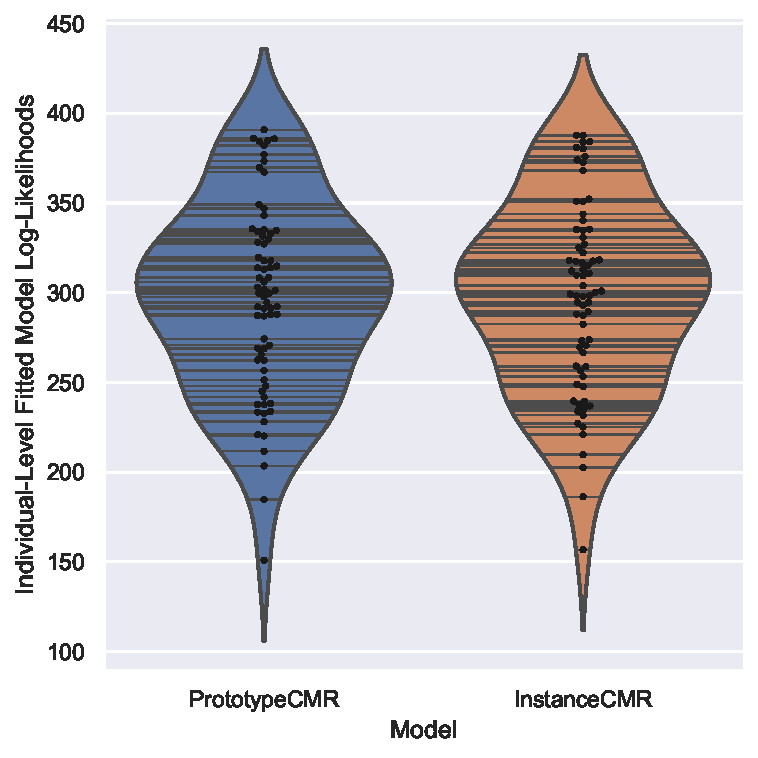
\includegraphics{./figures/individual_murdock1970.pdf}

}

\end{minipage}%
\newline
\begin{minipage}[c]{\linewidth}

{\centering 

\begin{longtable}[]{@{}lrr@{}}
\toprule()
& InstanceCMR & PrototypeCMR \\
\midrule()
\endhead
count & 72 & 72 \\
mean & 297.128 & 296.249 \\
std & 52.7989 & 52.8859 \\
min & 156.753 & 150.988 \\
25\% & 258.206 & 260.956 \\
50\% & 299.741 & 299.763 \\
75\% & 331.797 & 331.946 \\
max & 387.742 & 390.806 \\
\bottomrule()
\end{longtable}

}

\end{minipage}%

\caption{\label{fig-murdokafits}Distribution of log-likelihood scores of
recall sequences exhibited by each subject under each considered model
across list-lengths (Murdock \& Okada, 1970)}

\end{figure}

As a follow-up, we also compared how readily each model could account
for organizational summary statistics in the dataset. We found for each
model variant the optimal parameter configuration maximizing the
likelihood of the entire dataset rather than participant-by-participant.
Using each fitted model variant, we simulated 1000 unique free recall
trials and measured summary statistics from the result.
\textbf{?@fig-MurdOkaSummary} plots for each model against the
corresponding statistics collected over the dataset how recall
probability varies as a function of serial position, how the probability
of recalling an item first varies as a function of serial position, and
how the conditional recall probabability of an item varies as a function
of its serial lag from the previously recalled item. Recapitulating our
comparison of log-likelihood distributions fitted over discrete
participants, we found that both our prototype-based and instance-based
CMR implementations account for these benchmark organizational summary
statistics across the full dataset to similar extents. To build on this
finding of broad model equivalence with respect to the results reported
by Murdock \& Okada (1970), we consider the model variants under broader
experimental conditions.

\begin{figure}

{\centering 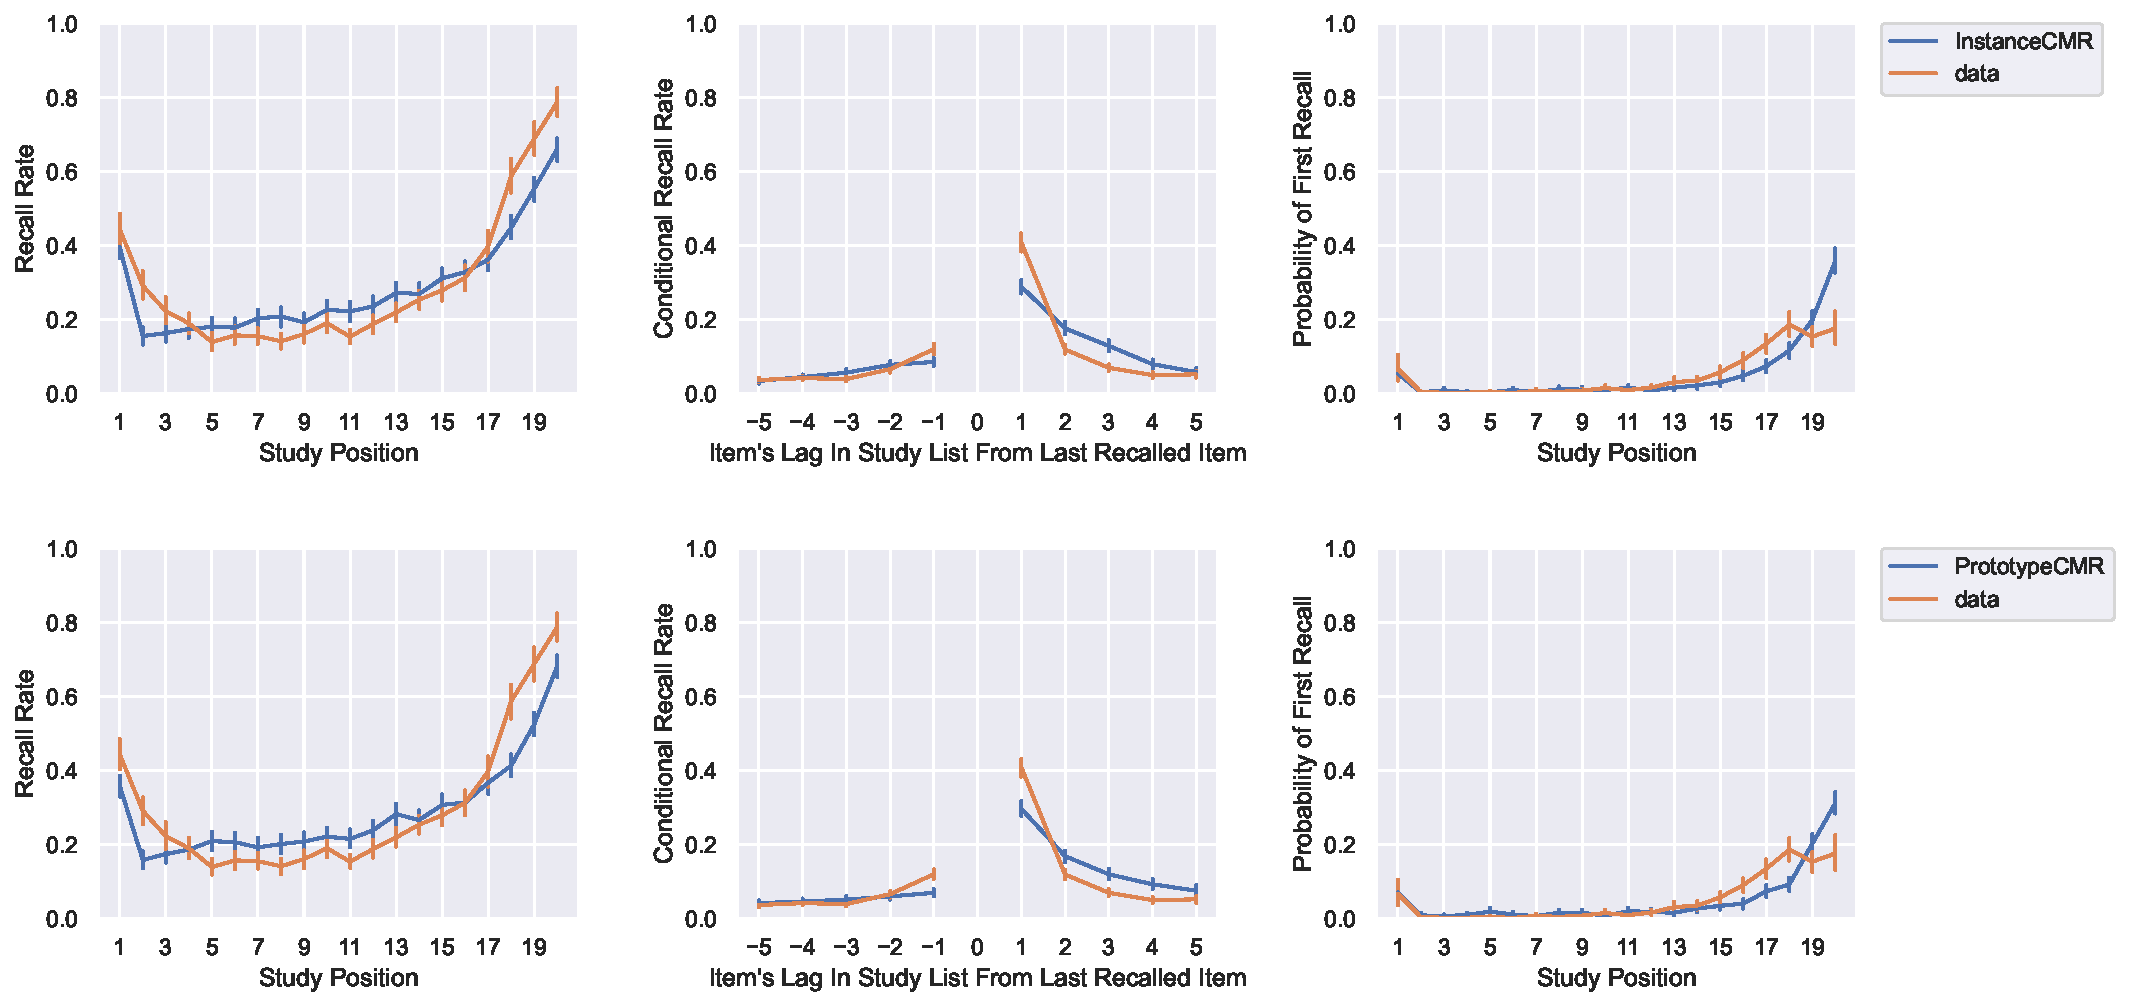
\includegraphics{./figures/overall_murdock1970.pdf}

}

\caption{\label{fig-murdokasummary}Comparison of summary statistics
between each model against observed data (Murdock \& Okada, 1970)}

\end{figure}

\hypertarget{simulation-of-murdock-jr-1962}{%
\section{Simulation of Murdock Jr
(1962)}\label{simulation-of-murdock-jr-1962}}

A significant feature of the context maintenance and retrieval (CMR)
model is its capacity to account for the relative scale-invariance of
serial position effects with respect to list length. Murdock Jr (1962)
found that changing list lengths across trials in a free recall
experiment impacted neither the shape of observed primacy effects during
recall nor on the slope of apparent recency effects, though other
features of recall sequences did change, such as the overall retrieval
probability for initially encoded items as well as the list-list
asymptote. Building on these observations, Polyn et al. (2009) found
that the CMR model could account for these effects of list length on the
shape of the serial position curve in free recall using a single
parameter configuration.

Here we investigate whether our prototype- and instance-based
implementations of CMR can similarly account for recall performance
across different list lengths when fitted to predict the sequences of
items recalled in our considered dataset. For these comparisons, we
leverage a subset of the original behavioral data reported by Murdock Jr
(1962). In the considered subset, 15 subjects performed 240 trials with
study lists each consisting of either 20, 30, or 40 unique words
presented sequentially -- 80 trials per list length.

For each model variant and each participant, we found through
differential evolution optimization the parameter configuration
maximizing the likelihood assigned by the model to each recall sequence
in all relevant trials, whether with list length of 20 or 30 or 40. The
log-likelihoods of the data corresponding to each participant and model
variant are plotted in \textbf{?@fig-Murd62Fits}, with a table providing
summary statistics. The distribution of log-likelihood scores between
participants for the PrototypeCMR and InstanceCMR model variants only
marginally differ, suggesting little meaningful difference between
variants in their effectiveness predicting recall sequences, even when
using a single parameter configuration per participant to account for
performance across variable list lengths.

\begin{figure}

\begin{minipage}[c]{\linewidth}

{\centering 

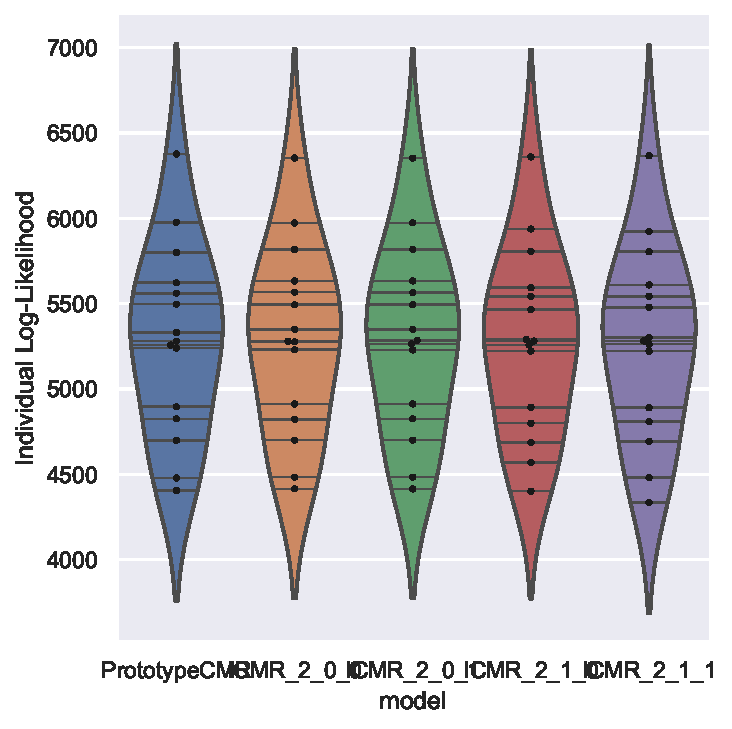
\includegraphics{./figures/individual_murdock1962.pdf}

}

\end{minipage}%
\newline
\begin{minipage}[c]{\linewidth}

{\centering 

\begin{longtable}[]{@{}lrr@{}}
\toprule()
& InstanceCMR & PrototypeCMR \\
\midrule()
\endhead
count & 15 & 15 \\
mean & 5300.61 & 5281.17 \\
std & 547.632 & 556.755 \\
min & 4475.97 & 4381.06 \\
25\% & 4873.37 & 4865.1 \\
50\% & 5300.33 & 5280.25 \\
75\% & 5620.59 & 5591.8 \\
max & 6382.21 & 6375.89 \\
\bottomrule()
\end{longtable}

}

\end{minipage}%

\caption{\label{fig-murdokafits}Distribution of log-likelihood scores of
recall sequences exhibited by each subject under each considered model
across list-lengths (Murdock Jr, 1962)}

\end{figure}

Considering log-likelihoods alone though leaves ambiguous whether the
influence of list length on serial position and related organizational
effects are effectively accounted for by both models. To find out, we
again focused scrutiny on the prototype-based and instance-based
implementations of CMR. We fit each model based on the likelihood
assigned to all recall sequences across the dataset rather than by
subject or list length. Summary statistics including recall probability
as a function of serial position, probability of first recall as a
function of serial position, and conditional recall probability as a
function of serial lag from the previously recalled item were computed
based on simulation of free recall data using the model variants with
their fitted parameters. Separate analyses simulated trials with study
list lengths of 20 and of 30 items, with summary statistics tracked
separately. \textbf{?@fig-Murd62Summary} plots the results of these
simulations against statistics from corresponding subsets of the
behavioral data from (Murdock Jr, 1962), with unique sets of plots for
both model variants and list lengths. As with previous analyses, we
found that both our prototype-based and instance-based CMR
implementations account for these benchmark organizational summary
statistics across the considered data to similar extents.

\begin{figure}

\begin{minipage}[t]{\linewidth}

{\centering 

\raisebox{-\height}{

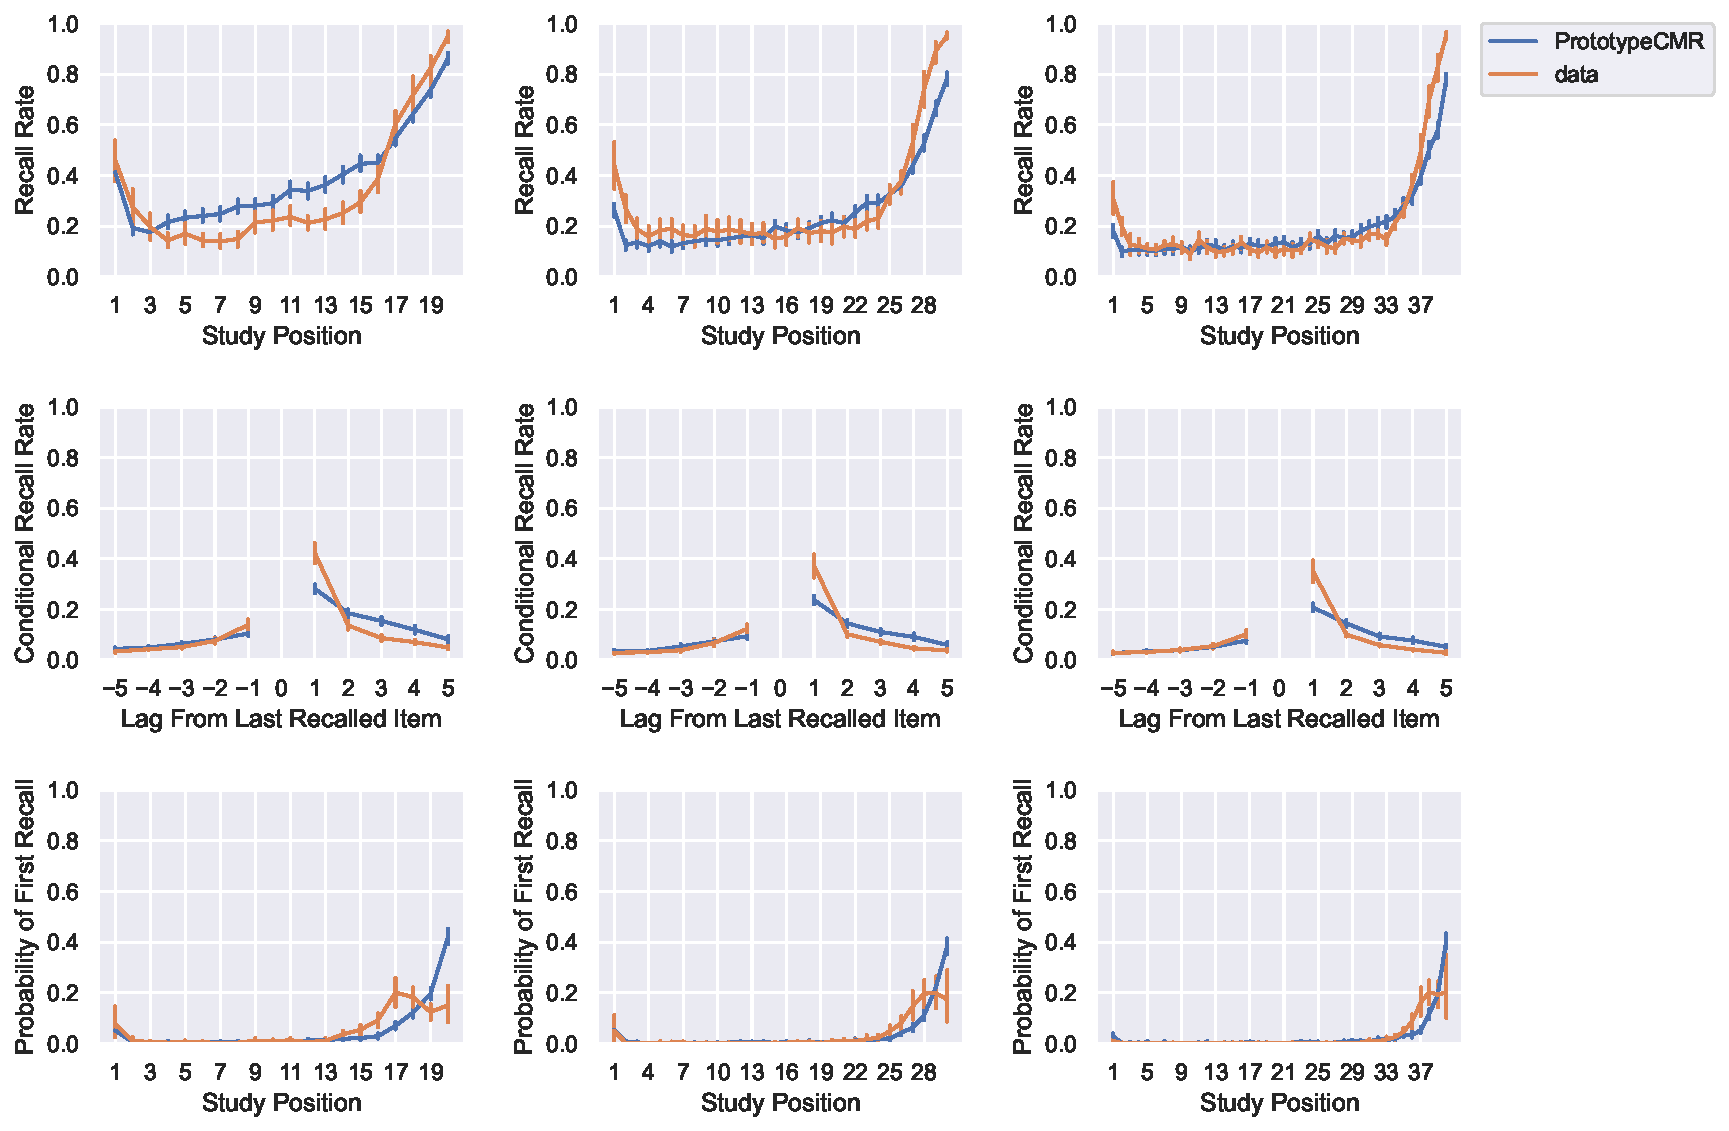
\includegraphics{./figures/cmr_summary_murdock1962.pdf}

}

}

\subcaption{\label{fig-PrototypeCMR}PrototypeCMR}
\end{minipage}%
\newline
\begin{minipage}[t]{\linewidth}

{\centering 

\raisebox{-\height}{

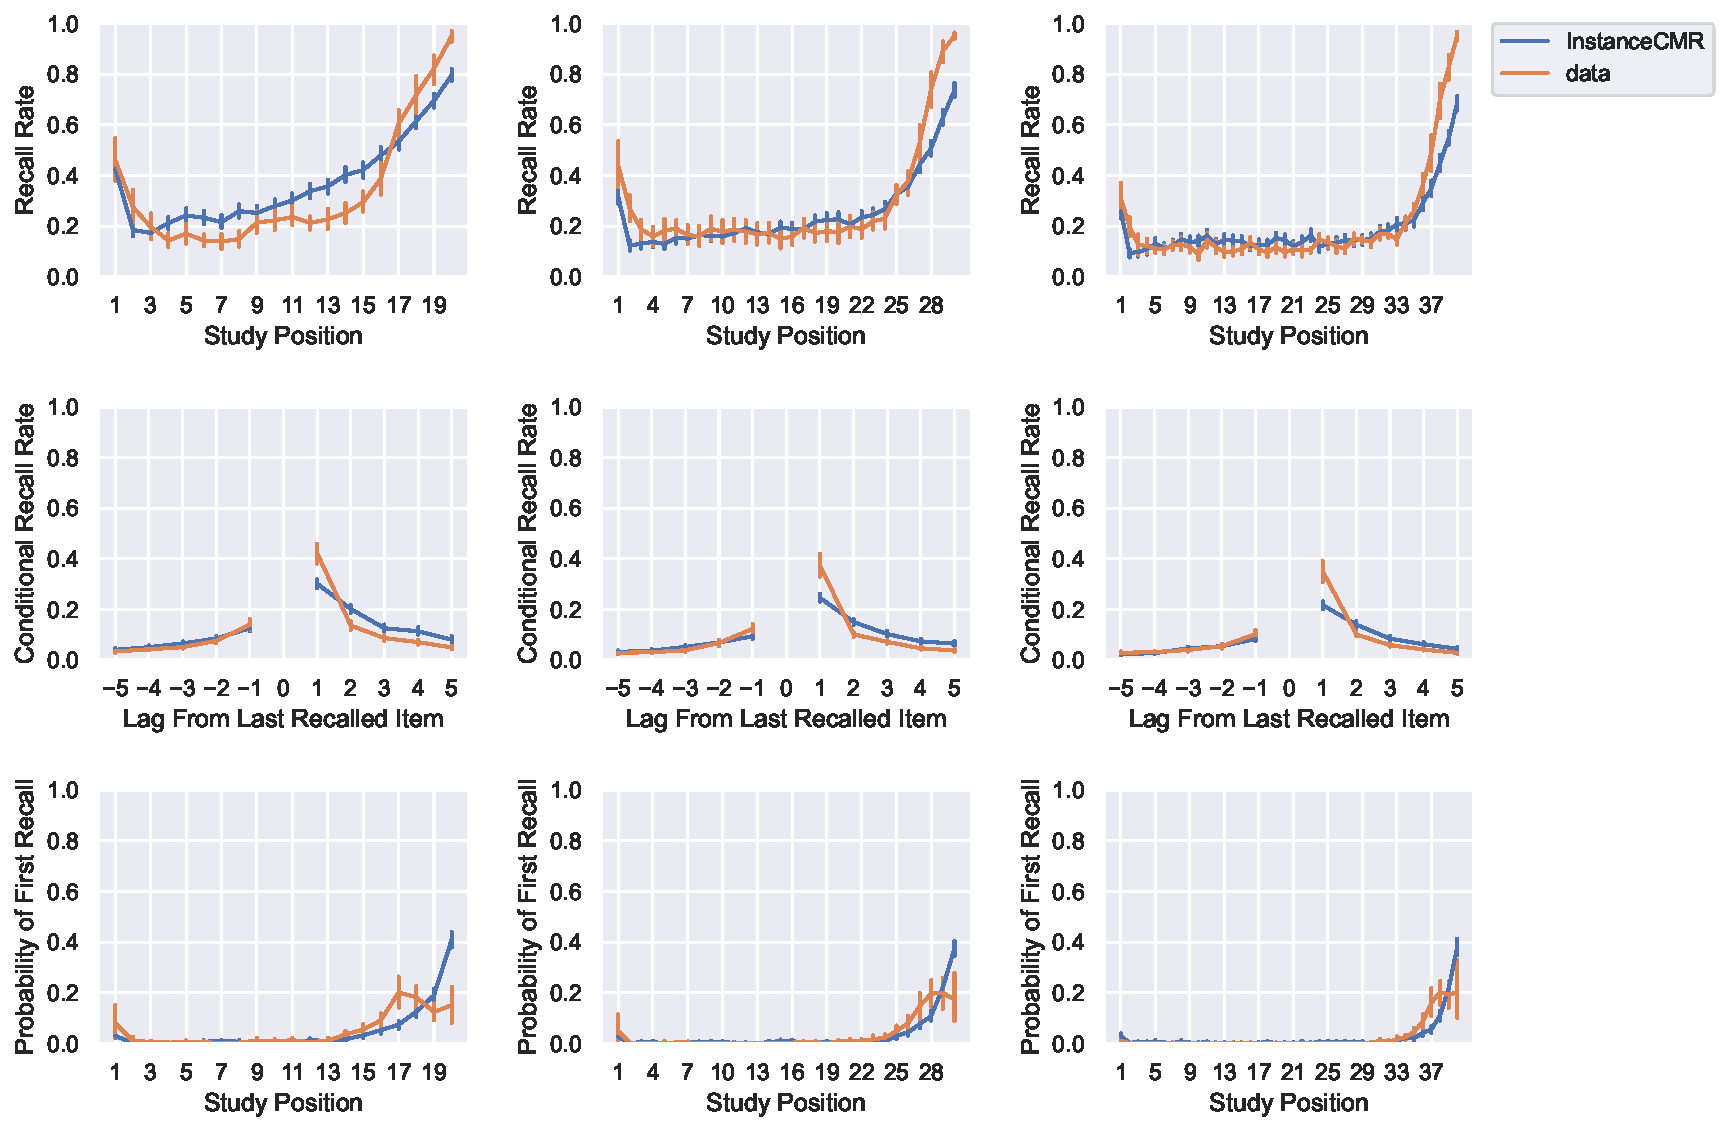
\includegraphics{./figures/icmr_summary_murdock1962.pdf}

}

}

\subcaption{\label{fig-InstanceCMR}InstanceCMR}
\end{minipage}%

\caption{\label{fig-murd62summary}Comparison of summary statistics
between each model against observed data (Murdock Jr, 1962)}

\end{figure}

\hypertarget{repetition-effects}{%
\section{Repetition Effects}\label{repetition-effects}}

While previous analyses evince that our prototype-based and
instance-based implementations of CMR equivalently account for free
recall performance when each unique item is presented just once during
study, there is reason to suspect that the models might diverge when it
comes to accounting for the effect of item repetition on later free
recall.

Previous work (Siegel \& Kahana, 2014) has related CMR to two broad
accounts of how item repetition influences memory and in particular
drives the spacing effect, a monotonic relationship between recall
probability and the size of the lag between item repetitions in a study
list. Under the contextual-variability account (Anderson \& Bower,
1972), each time an item is studied, it's associated in memory with the
current state of a slowly drifting contextual representation. Depending
on how spaced apart two presentations of an item might be, the
contextual states they are associated with might either be very similar
or very distinct. Later, participants use the current state of their
contextual representation to probe their memories and retrieve items
during free recall. When an item has been associated with diverse
contextual states, it can correspondingly be retrieved using diverse
possible cues. In this way, the improvements in recall we gain from
spacing presentations of an item are explained in terms of variation in
the range of possible cues that can trigger recall of that item. A
study-phase retrieval account of the spacing effect alternatively
emphasizes the consequences of studying a successively presented item.
According to the account, when this happens we retrieve memories of the
repeated item's earlier occurrences and their associated contexts. When
this happens, it's proposed that retrieved information is memorally
associated with information corresponding to the current presentation
context.

Analyses of our instance-based implementation of CMR so far suggest it
realizes these mechanisms similarly to the original prototype-based CMR.
A potentially more relevant distinction between the models might instead
turn on differences in how records of past experience are integrated for
retrieval. InstanceCMR, like MINERVA 2, has the option to apply its
nonlinear activation scaling parameter \(\tau\) to activations of
individual traces - that is, before integration into a unitary vector
tracking retrieval support. However, CMR does not access trace
activations and applies \(\tau\) to the integrated echo representation
result.

This distinction between instance-based and prototype-based
architectures has been marshalled to explain model differences in other
research contexts (e.g., Jamieson et al., 2018). In this context,
however, the different between applying \(\tau\) to trace activations or
echo content is between enforcing quasi-linear or quasi-exponential
effect of item repetition on subsequent recall probability. Suppose a
constant sensitivity parameter \(\tau\) and that two distinct
experiences each contributed a support of \(c\) for a given feature unit
in the current recall. Under trace-based sensitivity scaling, the
retrieval support for that feature unit would be
\(c^{\tau} + c^{\tau}\). But under echo-based sensitivity scaling,
support would be \({(c + c)}^{\tau}\), a much larger quantity.

Another way to illustrate this architectural difference is by
simulation. We can have our prototype-based and each variant of our
instance-based implementation of CMR simulate a traditional
list-learning experiment with study of 20 unique items in order. Then,
we can simulate repeated study of an arbitrary item in that list and
measure the effect on the probability of retrieving that item for each
successive repetition given a static retrieval cue.
Figure~\ref{fig-repeffect} plots the result of of this simulation over
1000 experiments for 50 item repetitions using PrototypeCMR and
InstanceCMRand model parameters fitted using data from Murdock \& Okada
(1970) and corresponds with our predictions. Model fitting over a
different dataset might obviate these observed differences; however
these simulations raise the possibility that with increasing item
repetitions, prototype-based and instance-based implementations of CMR
might support different predictions about the influence of item
repetition on later recall probability, motivating further
investigation.

\begin{figure}

\begin{minipage}[c]{0.50\linewidth}

{\centering 

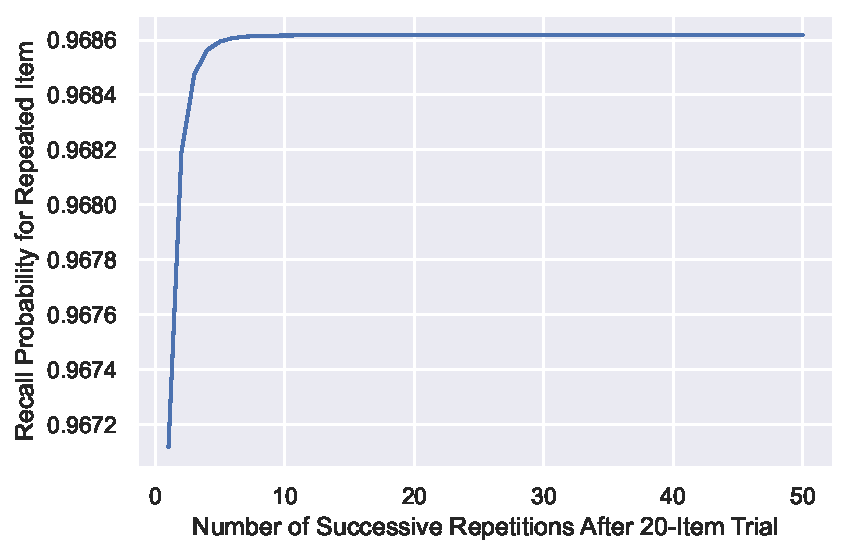
\includegraphics{./figures/cmr_repeffect.pdf}

}

\subcaption{\label{fig-cmr_repeffect}PrototypeCMR}
\end{minipage}%
%
\begin{minipage}[c]{0.50\linewidth}

{\centering 

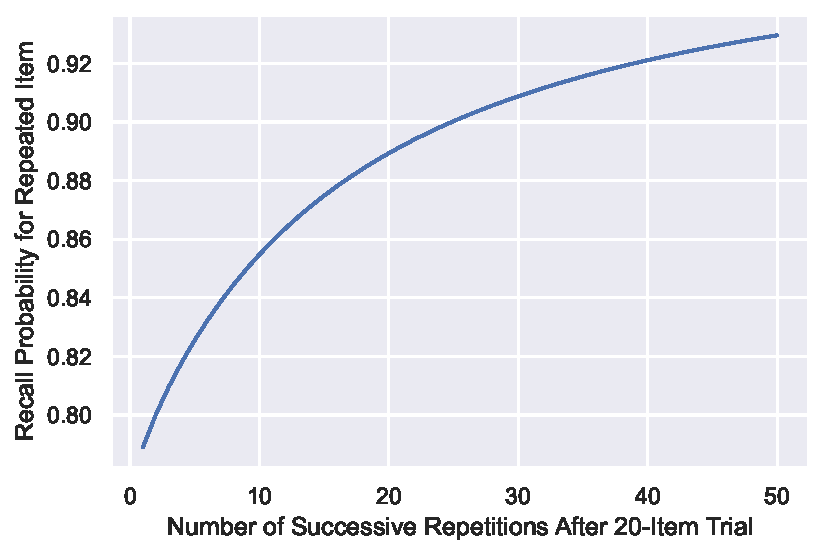
\includegraphics{./figures/icmr_repeffect.pdf}

}

\subcaption{\label{fig-icmr_repeffect}InstanceCMR}
\end{minipage}%

\caption{\label{fig-repeffect}Course of effect of successive item
repetitions on recall probability, by model, using parameters fitted
over Murdock \& Okada (1970) dataset and a static contextual cue after
simulation of a pure 20-item list.}

\end{figure}

Though initial simulations suggest a way to distinguish between
instance- and prototype-based accounts of context maintenance and
retrieval, free recall datasets with high amounts of repetition to the
extent simulated in the above example do not yet exist. However, to
support an initial comparison of how models account for item repetition
effects, we use data associated with Siegel \& Kahana (2014). Within the
dataset, 35 subjects performed delayed free recall of 48 lists over four
sessions. Except for deliberate item repetitions, words were unique
within each session and did not repeat in successive sessions. The
semantic relatedness of words was also controlled below a value of .55
according to WAS (Steyvers et al., 2005). Across trials, lists were
structured in four different ways:

\begin{enumerate}
\def\labelenumi{\arabic{enumi}.}
\item
  In control lists, all items were only presented once.
\item
  In pure massed lists, items were presented twice, always in succession
  (e.g.~1, 1, 2, 2)
\item
  In pure spaced lists, items were presented twice with spacing of
  repetitions from 1 to 8 positions, with each spacing amount
  equiprobable.
\item
  Finally, mixed lists feature once-presented, massed, and spaced items,
  with each spacing amount equiprobable
\end{enumerate}

As with previous analyses, each model variant was fit once for each
participant to identify the parameter configuration maximizing the
likelihood of observed recall sequences given the considered model,
considering all conditions of the dataset. The distribution of data
log-likelihoods given each fitted model and participant are plotted in
\textbf{?@fig-LohnasFits}, with median values for each model variant
highlighted. Similarly to previous analyses, these value distributions
were found largely similar. The distribution of log-likelihood scores
between participants for the PrototypeCMR and InstanceCMR model variants
only marginally differ, suggesting that all considered model variants
can predict recall sequences even when item repetitions occur during
study with similar degrees of success.

\begin{figure}

\begin{minipage}[c]{0.50\linewidth}

{\centering 

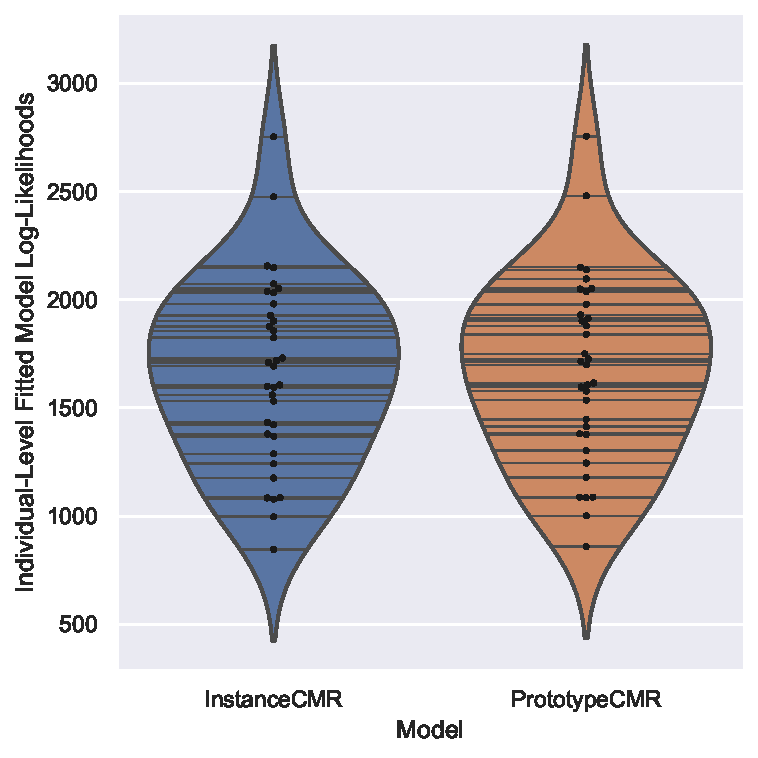
\includegraphics{./figures/individual_lohnas2014.pdf}

}

\end{minipage}%
%
\begin{minipage}[c]{0.50\linewidth}

{\centering 

\begin{longtable}[]{@{}lrr@{}}
\toprule()
& InstanceCMR & PrototypeCMR \\
\midrule()
\endhead
count & 35 & 35 \\
mean & 1676.3 & 1668.35 \\
std & 434.819 & 429.581 \\
min & 914.375 & 856.293 \\
25\% & 1367.75 & 1378.27 \\
50\% & 1686.97 & 1698.98 \\
75\% & 1955.37 & 1957.65 \\
max & 2752.36 & 2751.88 \\
\bottomrule()
\end{longtable}

}

\end{minipage}%

\caption{\label{fig-lohnasfits}Log-likelihood score distributions for
each subject under each considered model (Siegel \& Kahana, 2014)}

\end{figure}

While follow-up analysis of summary statistics in previous analyses
focused on benchmark phenomena such as serial position effects,
inclusion of item repetitions in study designs complicates associated
visualizations. Instead, we focused comparison on summary statistics
measuring classical item repetition effects. In
Figure~\ref{fig-lohnas_spacing}, we measure how effectively our
prototype- and instance-based CMR implementations account for the
spacing effect. Main model variants were fit to the mixed list (fourth)
condition of the entire dataset across subjects to optimize the
likelihood of observed recall sequences. Then with each configured
model, study phases of each trial in the mixed condition of the dataset
were simulated and then followed with simulation of free recall. We then
plot for both the behavioral data and simulated datasets, the rate at
which items were recalled, binned based on the number of intervening
items between repetitions. On the one hand, we observe that both models
poorly account for the pattern of recall rates observed as a function of
presentation spacing in the mixed condition of the Siegel \& Kahana
(2014) dataset, exaggerating the mnemonic benefit of item repetition in
general while understating the mnemonic effect of increased spacing
between repetitions. On the other hand, recapitulating all previous
analyses, we again found that both our prototype-based and main
instance-based implementations of CMR predicted similar patterns of
effects of repetition spacing on later item recall.

\begin{figure}

\begin{minipage}[t]{0.33\linewidth}

{\centering 

\raisebox{-\height}{

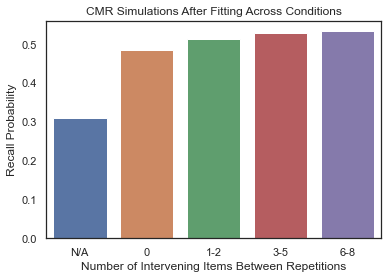
\includegraphics{./figures/cmr_spacing.png}

}

}

\subcaption{\label{fig-cmr_spacing}PrototypeCMR}
\end{minipage}%
%
\begin{minipage}[t]{0.33\linewidth}

{\centering 

\raisebox{-\height}{

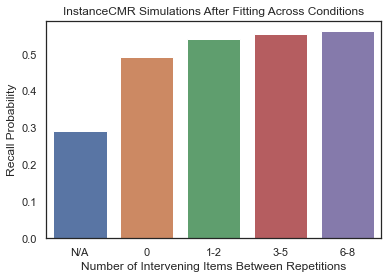
\includegraphics{./figures/icmr_spacing.png}

}

}

\subcaption{\label{fig-icmr_spacing}InstanceCMR}
\end{minipage}%
%
\begin{minipage}[t]{0.33\linewidth}

{\centering 

\raisebox{-\height}{

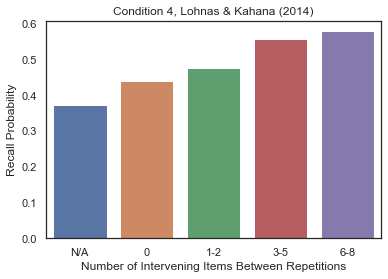
\includegraphics{./figures/data_spacing.png}

}

}

\subcaption{\label{fig-data_spacing}Data}
\end{minipage}%

\caption{\label{fig-lohnas_spacing}Comparison of predicted recall
probability as function of item repetition spacing between each model
and the observed data (Siegel \& Kahana, 2014).}

\end{figure}

\hypertarget{discussion}{%
\section{Discussion}\label{discussion}}

In light of a collection of results across task domains distinguishing
between the performance of prototype- and instance-based models of
memory-based behavior, we searched for evidence of a similar distinction
with respect to the free recall task paradigm. To do this, we specified
and compared the original prototype-based implementation of an
established model of task performance based in retrieved context theory
(PrototypeCMR) against a parallel instance-based variant (CMR) across
diverse experimental conditions, including a dataset featuring variable
study list lengths across trials and a dataset featuring item
repetitions within trials and variable item repetition spacing between
trials. While our simulation analyses focused on the effect of item
repetition on recall rates identified some hypothetical distinctions
between model predictions, the model variants accounted for human
performance on the free recall task with similar effectiveness in each
dataset considered.

One clear conclusion we can draw from these analyses is that the success
of the theoretical commitments made by the Context Maintenance and
Retrieval model and models like it are likely not especially dependent
on the architectures in which they are implemented. Instead, the main
insights of retrieved context theories (at least as formalized by CMR)
are highly portable, and can likely be esconced within any reasonable
model architecture where memory search via temporal contextual
representations might prove valuable. Establishing the portability of
these successful theoretical principles across modeling approaches helps
advance the historical effort in cognitive science to develop ``a
general account of memory and its processes in a working computational
system to produce a common explanation of behavior rather than a set of
lab-specific and domain-specific theories for different behaviors''
(Jamieson et al., 2018; Newell, 1973).

This finding has been increasingly validated lately in other work. Logan
(2021) for example similarly embeds mechanisms for maintaining and
organizing retrieval using temporal contextual representations within an
instance-based architecture to simultaneously account for performance on
substantively distinct variations of a task requiring participants to
encode and report random strings in left-to-right order by typing them
on a computer keyboard, including whole report, serial recall, and copy
typing. Other projects more motivated by neuroscientific data (e.g.
(Ketz et al., 2013); (Schapiro et al., 2017)) embed mechanisms for
context-based retrieval within detailed formal accounts of hippocampus
functionality more complex than either the instance-based or hebbian
associative network architectures considered in this work. Our
head-to-head comparison of this instance-based account of context
maintenance and retrieval against its more standard prototype-based
counterpart and observation that both competitively explain free recall
performance under varied conditions further evinces the architectural
independence of the retrieved context account of memory search.

How do these results fit into the context of other work identifying
substantive contrasts between instance- and prototype-based models?
Research by Jamieson et al. (2018) comparing the model architectures'
capacity to account for semantic memory emphasizes that the main
limitation of prototype-based models is the information that they
discard or distort toward some center-of-tendency at encoding -
idiosyncratic item or contextual features that do not reflect
generalities across experience. With this information discarded or
suppressed, memory cues selective for those idiosyncratic features
cannot result in retrieval of relevant information. Instance-based
models on the other hand are able to select information across learning
episodes to include in an abstractive representation based on the
content of a cue, enabling flexible retrieval of idiosyncratic features
while suppressing more common but irrelevant features.

The trace-based application of instance models' \(\tau\) parameter is
described as fundamental to the unique flexibility of instance-based
models outlined by Jamieson et al. (2018), as it enables instance-based
models to modulate the influence of particular memory traces in a
retrieved echo representation nonlinearly based on the traces'
similarity to a probe. However, while the prototype-based semantic
memory models examined by Jamieson et al. (2018) exclude a similar
response scaling mechanism, the standard prototype-based specification
of CMR does include one. Research on category learning (Nosofsky \&
Zaki, 2002; Stanton et al., 2002) also contrasting prototype- and
instance-based models of the behavior also identifies instance models'
characteristic response-scaling mechanism as crucial for accounting for
deterministic patterns in memory performance under various research
conditions. However, they also evaluate prototype-based models that,
like CMR, do include response-scaling mechanisms -- though by definition
only instance-based models apply the mechanism to similarities computed
between traces and probe representations. To compare the instance-based
Exemplar-Generalization model against a prototype-based model with a
similar response scaling mechanism, Nosofsky \& Zaki (2002) focused on
how the models differentially characterize generalization, in this case
the category assignment of novel items excluded from initial training.
Finding that participants mroe often classify items in the the same
categories based on their similarity to one another rather than based on
similarity to hypothetical prototype-representations, the instance-based
Exemplar-Generalization model came out ahead.

Even the research above drawing distinctions between the explanatory
performance of instance-based and prototype-based models report
experimental conditions where the two architectures perform similarly.
We can conclude that either the considered research conditions or the
model specifications themselves also sidestep any of their more
substantive differences. Two assumptions enforced in both the prototype-
and instance-based frameworks compared here as well as in corresponding
datasets were that list item were effectively representationally
orthogonal, and encountered just once or twice before retrieval.
Furthermore, contextual states as characterized by CMR differ a
consistent amount from item to item during study in a traditional list
learning experiment. The assumptions together may prevent a distinction
from emerging between highly common and highly idiosyncratic item or
contextual features under traditional research conditions as emphasized
in architectural comparisons drawn by Jamieson et al. (2018). Similarly,
the uniform similarity structure of list items studied and recalled
across evaluated datasets here potentially sidesteps issues raised by
Nosofsky \& Zaki (2002) with prototype-based models.

Higher rates of item repetition or enforced distortions of contextual
variation (such as by dividing an encoding phase into distinct trials or
sessions) might be enough to more clearly distinguish architecture
performance. Simulations of high rates of item repetitions reported in
Figure~\ref{fig-repeffect} identify one potentially relevant difference
between InstanceCMR and PrototypeCMR -- an exponential rate of increase
of recall rates for repeated items in the former, but not the latter --
but the distinction seems independent from contrasts drawn between the
architectures drawn by other researchers such as Jamieson et al. (2018)
and Nosofsky \& Zaki (2002). By contrast, research conditions where
items are repeated rarely in some contexts but frequently in others or
nonorthogonal item features influence and are factored into model
performance would further explore the relevance of prior exploration of
prototype- and instance-based architectures to our understanding of free
recall and similar tasks. At the same time, our current results
establish that architectural distinctions relevant in other tasks
domains may be not particularly critical for accounting for performance
across the more traditional research conditions explored here.

While these results suggest some level of equivalance between
instance-based and prototype-based models with respect to accounting for
free recall performance, their generality is as limited to the simple
architectures evaluated as to the datasets explored. More complex or
just different models that might be classed in one of these categories
may not exhibit the same patterns. For example, the examinations here
only consider a constrained conceptualization of instance-based models
styled after the MINERVA 2 simulation model of human memory (Hintzman,
1984). Lehman \& Malmberg (2013) produced a dual store model of
performance on various recall tasks and can be classed as an
instance-based model despite excluding some traditional features of
models inspired by Hintzman (1984), such as reliance on a single trace
store and application of a nonlinear response scaling mechanism during
retrieval. Its main assumption is that a limited-capacity buffer tracks
both information about items and about associations between items and
between items and their encoding context; at the same time, it supposes
that a secondary, unlimited-capacity store is, with some probability,
populated with traces from this buffer. For the free recall task, the
model integrates concepts from retrieved context theory, including
initiation of recall based on the content of a context cue. With these
mechanisms, the model is able to account for serial position and
temporal contiguity effects using novel mechanisms not directly
instantiated in the variants of CMR explored here. Similarities in
predictions offered by the different models indicate that they include
analogous features, but important explanatory differences may just as
well exist between them and MINERVA-based instance models under certain
research conditions as exist between prototype-based and instance-based
models in others. Deeper clarification of the distinctions and
homologies between different models characterizing performance on memory
tasks such as free recall is critical for driving further modeling
innovation.

\hypertarget{references}{%
\section{References}\label{references}}

\hypertarget{refs}{}
\begin{CSLReferences}{1}{0}
\leavevmode\vadjust pre{\hypertarget{ref-anderson1972recognition}{}}%
Anderson, J. R., \& Bower, G. H. (1972). Recognition and retrieval
processes in free recall. \emph{Psychological Review}, \emph{79}(2), 97.

\leavevmode\vadjust pre{\hypertarget{ref-church2017word2vec}{}}%
Church, K. W. (2017). Word2Vec. \emph{Natural Language Engineering},
\emph{23}(1), 155--162.

\leavevmode\vadjust pre{\hypertarget{ref-dumais2004latent}{}}%
Dumais, S. T. (2004). Latent semantic analysis. \emph{Annual Review of
Information Science and Technology}, \emph{38}(1), 188--230.

\leavevmode\vadjust pre{\hypertarget{ref-friendly1982toronto}{}}%
Friendly, M., Franklin, P. E., Hoffman, D., \& Rubin, D. C. (1982). The
toronto word pool: Norms for imagery, concreteness, orthographic
variables, and grammatical usage for 1,080 words. \emph{Behavior
Research Methods \& Instrumentation}, \emph{14}(4), 375--399.

\leavevmode\vadjust pre{\hypertarget{ref-golomb2008effects}{}}%
Golomb, J. D., Peelle, J. E., Addis, K. M., Kahana, M. J., \& Wingfield,
A. (2008). Effects of adult aging on utilization of temporal and
semantic associations during free and serial recall. \emph{Memory \&
Cognition}, \emph{36}(5), 947--956.

\leavevmode\vadjust pre{\hypertarget{ref-healey2016four}{}}%
Healey, M. K., \& Kahana, M. J. (2016). A four-component model of
age-related memory change. \emph{Psychological Review}, \emph{123}(1),
23.

\leavevmode\vadjust pre{\hypertarget{ref-hintzman1984minerva}{}}%
Hintzman, D. L. (1984). MINERVA 2: A simulation model of human memory.
\emph{Behavior Research Methods, Instruments, \& Computers},
\emph{16}(2), 96--101.

\leavevmode\vadjust pre{\hypertarget{ref-hintzman1986schema}{}}%
Hintzman, D. L. (1986). "Schema abstraction" in a multiple-trace memory
model. \emph{Psychological Review}, \emph{93}(4), 411.

\leavevmode\vadjust pre{\hypertarget{ref-hintzman1988judgments}{}}%
Hintzman, D. L. (1988). Judgments of frequency and recognition memory in
a multiple-trace memory model. \emph{Psychological Review},
\emph{95}(4), 528.

\leavevmode\vadjust pre{\hypertarget{ref-howard2002distributed}{}}%
Howard, M. W., \& Kahana, M. J. (2002). A distributed representation of
temporal context. \emph{Journal of Mathematical Psychology},
\emph{46}(3), 269--299.

\leavevmode\vadjust pre{\hypertarget{ref-jamieson2018instance}{}}%
Jamieson, R. K., Avery, J. E., Johns, B. T., \& Jones, M. N. (2018). An
instance theory of semantic memory. \emph{Computational Brain \&
Behavior}, \emph{1}(2), 119--136.

\leavevmode\vadjust pre{\hypertarget{ref-kahana1996associative}{}}%
Kahana, M. J. (1996). Associative retrieval processes in free recall.
\emph{Memory \& Cognition}, \emph{24}(1), 103--109.

\leavevmode\vadjust pre{\hypertarget{ref-kahana2020computational}{}}%
Kahana, M. J. (2020). Computational models of memory search.
\emph{Annual Review of Psychology}, \emph{71}, 107--138.

\leavevmode\vadjust pre{\hypertarget{ref-ketz2013theta}{}}%
Ketz, N., Morkonda, S. G., \& O'Reilly, R. C. (2013). Theta coordinated
error-driven learning in the hippocampus. \emph{PLoS Comput Biol},
\emph{9}(6), e1003067.

\leavevmode\vadjust pre{\hypertarget{ref-kragel2015neural}{}}%
Kragel, J. E., Morton, N. W., \& Polyn, S. M. (2015). Neural activity in
the medial temporal lobe reveals the fidelity of mental time travel.
\emph{Journal of Neuroscience}, \emph{35}(7), 2914--2926.

\leavevmode\vadjust pre{\hypertarget{ref-lehman2013buffer}{}}%
Lehman, M., \& Malmberg, K. J. (2013). A buffer model of memory encoding
and temporal correlations in retrieval. \emph{Psychological Review},
\emph{120}(1), 155.

\leavevmode\vadjust pre{\hypertarget{ref-logan2021serial}{}}%
Logan, G. D. (2021). Serial order in perception, memory, and action.
\emph{Psychological Review}, \emph{128}(1), 1.

\leavevmode\vadjust pre{\hypertarget{ref-morton2016predictive}{}}%
Morton, N. W., \& Polyn, S. M. (2016). A predictive framework for
evaluating models of semantic organization in free recall. \emph{Journal
of Memory and Language}, \emph{86}, 119--140.

\leavevmode\vadjust pre{\hypertarget{ref-murdock1970interresponse}{}}%
Murdock, B. B., \& Okada, R. (1970). Interresponse times in single-trial
free recall. \emph{Journal of Experimental Psychology}, \emph{86}(2),
263.

\leavevmode\vadjust pre{\hypertarget{ref-murdock1962serial}{}}%
Murdock Jr, B. B. (1962). The serial position effect of free recall.
\emph{Journal of Experimental Psychology}, \emph{64}(5), 482.

\leavevmode\vadjust pre{\hypertarget{ref-newell1973you}{}}%
Newell, A. (1973). \emph{You can't play 20 questions with nature and
win: Projective comments on the papers of this symposium}.

\leavevmode\vadjust pre{\hypertarget{ref-nosofsky2002exemplar}{}}%
Nosofsky, R. M., \& Zaki, S. R. (2002). Exemplar and prototype models
revisited: Response strategies, selective attention, and stimulus
generalization. \emph{Journal of Experimental Psychology: Learning,
Memory, and Cognition}, \emph{28}(5), 924.

\leavevmode\vadjust pre{\hypertarget{ref-polyn2009context}{}}%
Polyn, S. M., Norman, K. A., \& Kahana, M. J. (2009). A context
maintenance and retrieval model of organizational processes in free
recall. \emph{Psychological Review}, \emph{116}(1), 129.

\leavevmode\vadjust pre{\hypertarget{ref-postman1971organization}{}}%
Postman, L. (1971). Organization and interference. \emph{Psychological
Review}, \emph{78}(4), 290.

\leavevmode\vadjust pre{\hypertarget{ref-puff1979memory}{}}%
Puff, C. R. (1979). \emph{Memory organization and structure}. Academic
Press.

\leavevmode\vadjust pre{\hypertarget{ref-schapiro2017complementary}{}}%
Schapiro, A. C., Turk-Browne, N. B., Botvinick, M. M., \& Norman, K. A.
(2017). Complementary learning systems within the hippocampus: A neural
network modelling approach to reconciling episodic memory with
statistical learning. \emph{Philosophical Transactions of the Royal
Society B: Biological Sciences}, \emph{372}(1711), 20160049.

\leavevmode\vadjust pre{\hypertarget{ref-schwartz2005shadows}{}}%
Schwartz, G., Howard, M. W., Jing, B., \& Kahana, M. J. (2005). Shadows
of the past: Temporal retrieval effects in recognition memory.
\emph{Psychological Science}, \emph{16}(11), 898--904.

\leavevmode\vadjust pre{\hypertarget{ref-siegel2014retrieved}{}}%
Siegel, L. L., \& Kahana, M. J. (2014). A retrieved context account of
spacing and repetition effects in free recall. \emph{Journal of
Experimental Psychology: Learning, Memory, and Cognition}, \emph{40}(3),
755.

\leavevmode\vadjust pre{\hypertarget{ref-stanton2002comparisons}{}}%
Stanton, R. D., Nosofsky, R. M., \& Zaki, S. R. (2002). Comparisons
between exemplar similarity and mixed prototype models using a linearly
separable category structure. \emph{Memory \& Cognition}, \emph{30}(6),
934--944.

\leavevmode\vadjust pre{\hypertarget{ref-steyvers2005word}{}}%
Steyvers, M., Shiffrin, R. M., \& Nelson, D. L. (2005). \emph{Word
association spaces for predicting semantic similarity effects in
episodic memory.}

\leavevmode\vadjust pre{\hypertarget{ref-storn1997differential}{}}%
Storn, R., \& Price, K. (1997). Differential evolution--a simple and
efficient heuristic for global optimization over continuous spaces.
\emph{Journal of Global Optimization}, \emph{11}(4), 341--359.

\leavevmode\vadjust pre{\hypertarget{ref-talmi2019retrieved}{}}%
Talmi, D., Lohnas, L. J., \& Daw, N. D. (2019). A retrieved context
model of the emotional modulation of memory. \emph{Psychological
Review}, \emph{126}(4), 455.

\leavevmode\vadjust pre{\hypertarget{ref-wachter2019retrieved}{}}%
Wachter, J. A., \& Kahana, M. J. (2019). \emph{A retrieved-context
theory of financial decisions}. National Bureau of Economic Research.

\leavevmode\vadjust pre{\hypertarget{ref-yee2019abstraction}{}}%
Yee, E. (2019). \emph{Abstraction and concepts: When, how, where, what
and why?} Taylor \& Francis.

\end{CSLReferences}



\end{document}
